% "What the network sees" with measured motor speeds, for the A1 poster.
% One source, two figures (set \histlen before \input):
%   pdflatex -jobname=fig_inputs_short_poster "\def\histlen{4}% "What the network sees" with measured motor speeds, for the A1 poster.
% One source, two figures (set \histlen before \input):
%   pdflatex -jobname=fig_inputs_short_poster "\def\histlen{4}% "What the network sees" with measured motor speeds, for the A1 poster.
% One source, two figures (set \histlen before \input):
%   pdflatex -jobname=fig_inputs_short_poster "\def\histlen{4}% "What the network sees" with measured motor speeds, for the A1 poster.
% One source, two figures (set \histlen before \input):
%   pdflatex -jobname=fig_inputs_short_poster "\def\histlen{4}\input{fig_inputs_rpm_poster.tex}"   (41 inputs)
%   pdflatex -jobname=fig_inputs_none_poster  "\def\histlen{0}\input{fig_inputs_rpm_poster.tex}"   (25 inputs)
% Compiled on its own it gives the 4-step version. In the poster:
%   \includegraphics[width=\linewidth]{images/fig_inputs_short_poster.pdf}
\documentclass[12pt, border=4pt]{standalone}
\usepackage{tikz}
\usetikzlibrary{arrows.meta,positioning,calc,decorations.pathreplacing}
\renewcommand{\familydefault}{\sfdefault}

\definecolor{saclaydk}{RGB}{27,67,32}
\definecolor{mandarine}{RGB}{243,115,32}
\definecolor{vert}{RGB}{140,198,62}
\definecolor{bleu}{RGB}{80,144,205}
\definecolor{rouge}{RGB}{198,11,70}

\tikzset{
  cell/.style={draw=#1!70!black, fill=#1!45, line width=0.6pt},
  card/.style={draw=#1, fill=#1!10, rounded corners=4pt, line width=1.4pt},
  arr/.style={-{Stealth[length=4mm,width=3mm]}, line width=2pt},
}
\newcommand{\s}{0.36} % cell size
\providecommand{\histlen}{4}

\begin{document}
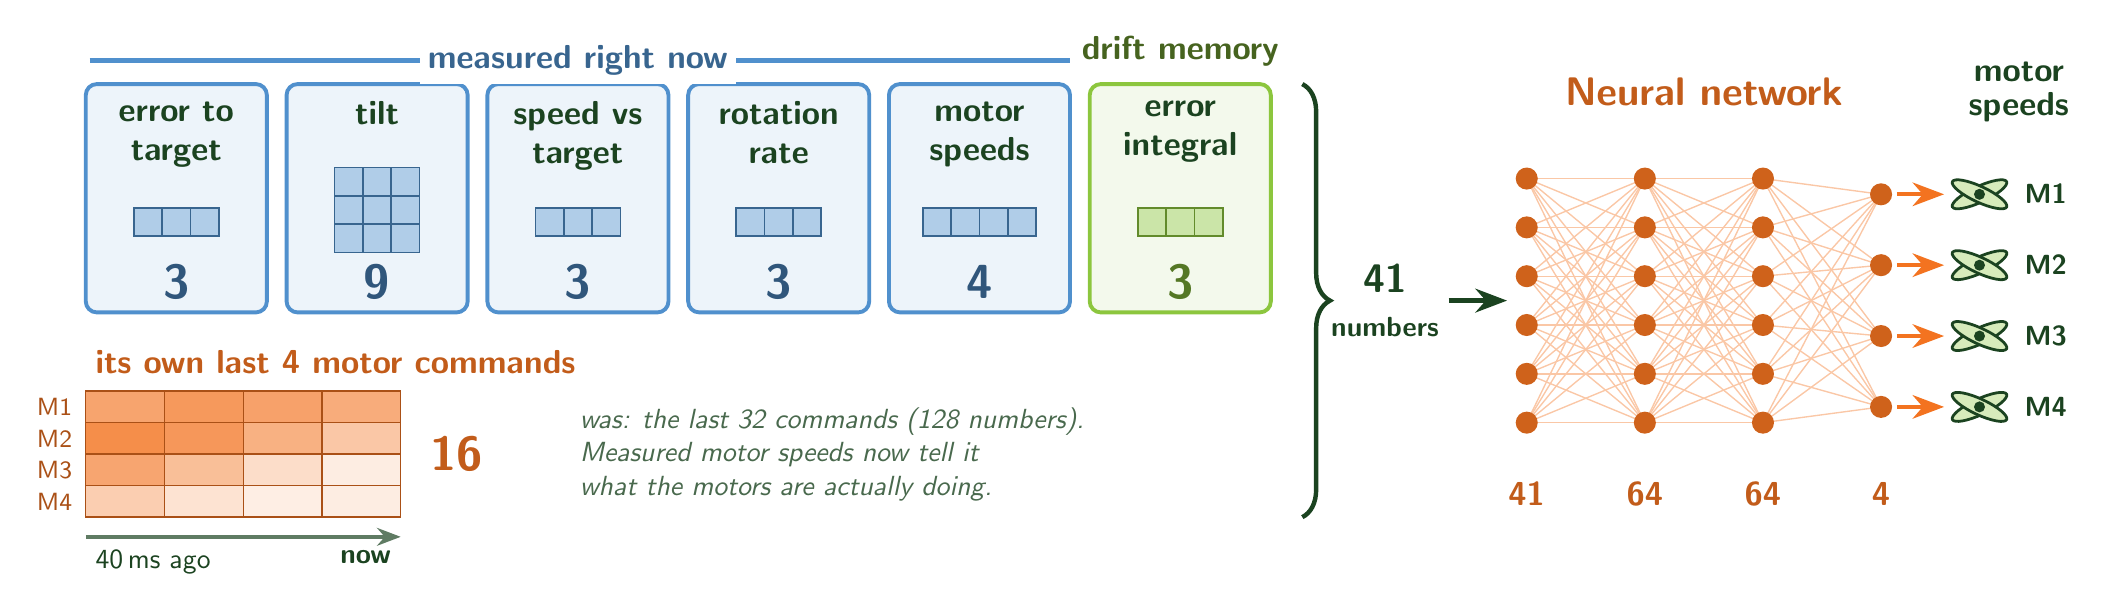
\begin{tikzpicture}
  % ---------- the "right now" groups as cards ----------
  \foreach \x/\ttl/\n/\col in {
      0/{error to\\target}/3/bleu,
      2.55/{tilt}/9/bleu,
      5.1/{speed vs\\target}/3/bleu,
      7.65/{rotation\\rate}/3/bleu,
      10.2/{motor\\speeds}/4/bleu,
      12.75/{error\\integral}/3/vert} {
    \draw[card=\col] (\x-1.15,-1.45) rectangle (\x+1.15,1.45);
    \node[align=center, font=\large\bfseries, text=saclaydk, anchor=north] at (\x,1.35) {\ttl};
    \node[font=\LARGE\bfseries, text=\col!60!black, anchor=south] at (\x,-1.4) {\n};
  }
  % cells inside the cards
  \foreach \x in {0,5.1,7.65} \foreach \i in {-1,0,1}
    \draw[cell=bleu] (\x+\i*\s-\s/2,-0.3-\s/2) rectangle ++(\s,\s);
  \foreach \i in {-1,0,1} \foreach \j in {-1,0,1}
    \draw[cell=bleu] (2.55+\i*\s-\s/2,-0.15+\j*\s-\s/2) rectangle ++(\s,\s);
  \foreach \i in {-1.5,-0.5,0.5,1.5}
    \draw[cell=bleu] (10.2+\i*\s-\s/2,-0.3-\s/2) rectangle ++(\s,\s);
  \foreach \i in {-1,0,1}
    \draw[cell=vert] (12.75+\i*\s-\s/2,-0.3-\s/2) rectangle ++(\s,\s);

  % group headers
  \draw[bleu, line width=1.6pt] (-1.1,1.75) -- (11.35,1.75);
  \node[font=\large\bfseries, text=bleu!70!black, fill=white, inner sep=3pt] at (5.1,1.75) {measured right now};
  \node[font=\large\bfseries, text=vert!50!black, anchor=south] at (12.75,1.55) {drift memory};

  \ifnum\histlen>0
    % ---------- memory: its own last few commands ----------
    \pgfmathtruncatemacro{\nh}{\histlen}
    \pgfmathtruncatemacro{\nnum}{4*\histlen}
    \pgfmathtruncatemacro{\ms}{10*\histlen}
    \def\gw{1.0}
    \node[anchor=south west, font=\large\bfseries, text=mandarine!80!black] at (-1.15,-2.35)
         {its own last \nh\ motor commands};
    \foreach \c in {1,...,\nh} \foreach \r in {0,...,3} {
      \pgfmathtruncatemacro{\v}{max(12, min(85, 45 + 25*sin(\c*23 + \r*70) + 12*sin(\c*61 + \r*20)))}
      \draw[draw=mandarine!70!black, line width=0.5pt, fill=mandarine!\v]
        (-1.15+\c*\gw-\gw, -2.45-\r*0.4) rectangle ++(\gw, -0.4);
    }
    \node[anchor=west, font=\LARGE\bfseries, text=mandarine!80!black] at (-1.15+\nh*\gw+0.25,-3.25) {\nnum};
    \foreach \r/\m in {0/1,1/2,2/3,3/4}
      \node[font=\small, text=mandarine!70!black, anchor=east] at (-1.2,-2.65-\r*0.4) {M\m};
    \draw[-{Stealth[length=3mm]}, line width=1.4pt, saclaydk!70] (-1.15,-4.3) -- (-1.15+\nh*\gw,-4.3);
    \node[anchor=north west, font=\normalsize, text=saclaydk] at (-1.15,-4.35) {\ms\,ms ago};
    \node[anchor=north east, font=\normalsize\bfseries, text=saclaydk] at (-1.15+\nh*\gw,-4.35) {now};
    \node[anchor=west, align=left, font=\normalsize\itshape, text=saclaydk!80] at (5.0,-3.25)
         {was: the last 32 commands (128 numbers).\\Measured motor speeds now tell it\\what the motors are actually doing.};
    \def\ybot{-4.05}
    \def\ny{-1.3}
  \else
    \node[anchor=north west, align=left, font=\normalsize\itshape, text=saclaydk!80] at (-1.15,-1.8)
         {No memory of its own commands (was: the last 32 = 128 numbers).\\
          Measured motor speeds tell it what the motors are actually doing.};
    \def\ybot{-1.45}
    \def\ny{0}
  \fi
  \pgfmathtruncatemacro{\total}{22 + 4*\histlen + 3}

  % ---------- bracket into the network ----------
  \draw[decorate, decoration={brace, amplitude=10pt}, line width=1.6pt, saclaydk]
    (14.3,1.45) -- (14.3,\ybot);
  \node[font=\Large\bfseries, text=saclaydk, align=center] (tot) at (15.35,\ny) {\total\\[-2pt]{\normalsize numbers}};
  \draw[arr, saclaydk] (tot.east) -- (16.9,\ny);

  % ---------- network ----------
  \pgfmathtruncatemacro{\nin}{\histlen > 0 ? 6 : 5}
  \foreach \L/\x/\n/\sp in {0/17.15/\nin/0.62, 1/18.65/6/0.62, 2/20.15/6/0.62, 3/21.65/4/0.9} {
    \foreach \k in {1,...,\n} \coordinate (N\L-\k) at (\x, {\ny + (\n+1)/2*\sp - \k*\sp});
  }
  \foreach \a/\na/\b/\nb in {0/\nin/1/6, 1/6/2/6, 2/6/3/4}
    \foreach \i in {1,...,\na} \foreach \j in {1,...,\nb}
      \draw[mandarine!40, line width=0.5pt] (N\a-\i) -- (N\b-\j);
  \foreach \L/\n in {0/\nin,1/6,2/6,3/4} \foreach \k in {1,...,\n}
    \fill[mandarine!85!black] (N\L-\k) circle (0.14);
  \foreach \x/\lab in {17.15/\total, 18.65/64, 20.15/64, 21.65/4}
    \node[font=\large\bfseries, text=mandarine!80!black] at (\x,\ny-2.45) {\lab};
  \node[font=\Large\bfseries, text=mandarine!80!black] at (19.4,\ny+2.65) {Neural network};

  % ---------- outputs: 4 propellers ----------
  \foreach \k in {1,...,4} {
    \coordinate (P) at ($(N3-\k)+(1.25,0)$);
    \draw[arr, mandarine, line width=1.4pt] ($(N3-\k)+(0.2,0)$) -- ($(P)+(-0.45,0)$);
    \draw[saclaydk, fill=vert!35, line width=1pt, rotate around={25:(P)}] (P) ellipse (0.38 and 0.1);
    \draw[saclaydk, fill=vert!35, line width=1pt, rotate around={-25:(P)}] (P) ellipse (0.38 and 0.1);
    \fill[saclaydk] (P) circle (0.07);
    \node[anchor=west, font=\normalsize\bfseries, text=saclaydk] at ($(P)+(0.45,0)$) {M\k};
  }
  \node[align=center, font=\large\bfseries, text=saclaydk] at (23.4,\ny+2.65) {motor\\[-2pt]speeds};
\end{tikzpicture}
\end{document}
"   (41 inputs)
%   pdflatex -jobname=fig_inputs_none_poster  "\def\histlen{0}% "What the network sees" with measured motor speeds, for the A1 poster.
% One source, two figures (set \histlen before \input):
%   pdflatex -jobname=fig_inputs_short_poster "\def\histlen{4}\input{fig_inputs_rpm_poster.tex}"   (41 inputs)
%   pdflatex -jobname=fig_inputs_none_poster  "\def\histlen{0}\input{fig_inputs_rpm_poster.tex}"   (25 inputs)
% Compiled on its own it gives the 4-step version. In the poster:
%   \includegraphics[width=\linewidth]{images/fig_inputs_short_poster.pdf}
\documentclass[12pt, border=4pt]{standalone}
\usepackage{tikz}
\usetikzlibrary{arrows.meta,positioning,calc,decorations.pathreplacing}
\renewcommand{\familydefault}{\sfdefault}

\definecolor{saclaydk}{RGB}{27,67,32}
\definecolor{mandarine}{RGB}{243,115,32}
\definecolor{vert}{RGB}{140,198,62}
\definecolor{bleu}{RGB}{80,144,205}
\definecolor{rouge}{RGB}{198,11,70}

\tikzset{
  cell/.style={draw=#1!70!black, fill=#1!45, line width=0.6pt},
  card/.style={draw=#1, fill=#1!10, rounded corners=4pt, line width=1.4pt},
  arr/.style={-{Stealth[length=4mm,width=3mm]}, line width=2pt},
}
\newcommand{\s}{0.36} % cell size
\providecommand{\histlen}{4}

\begin{document}
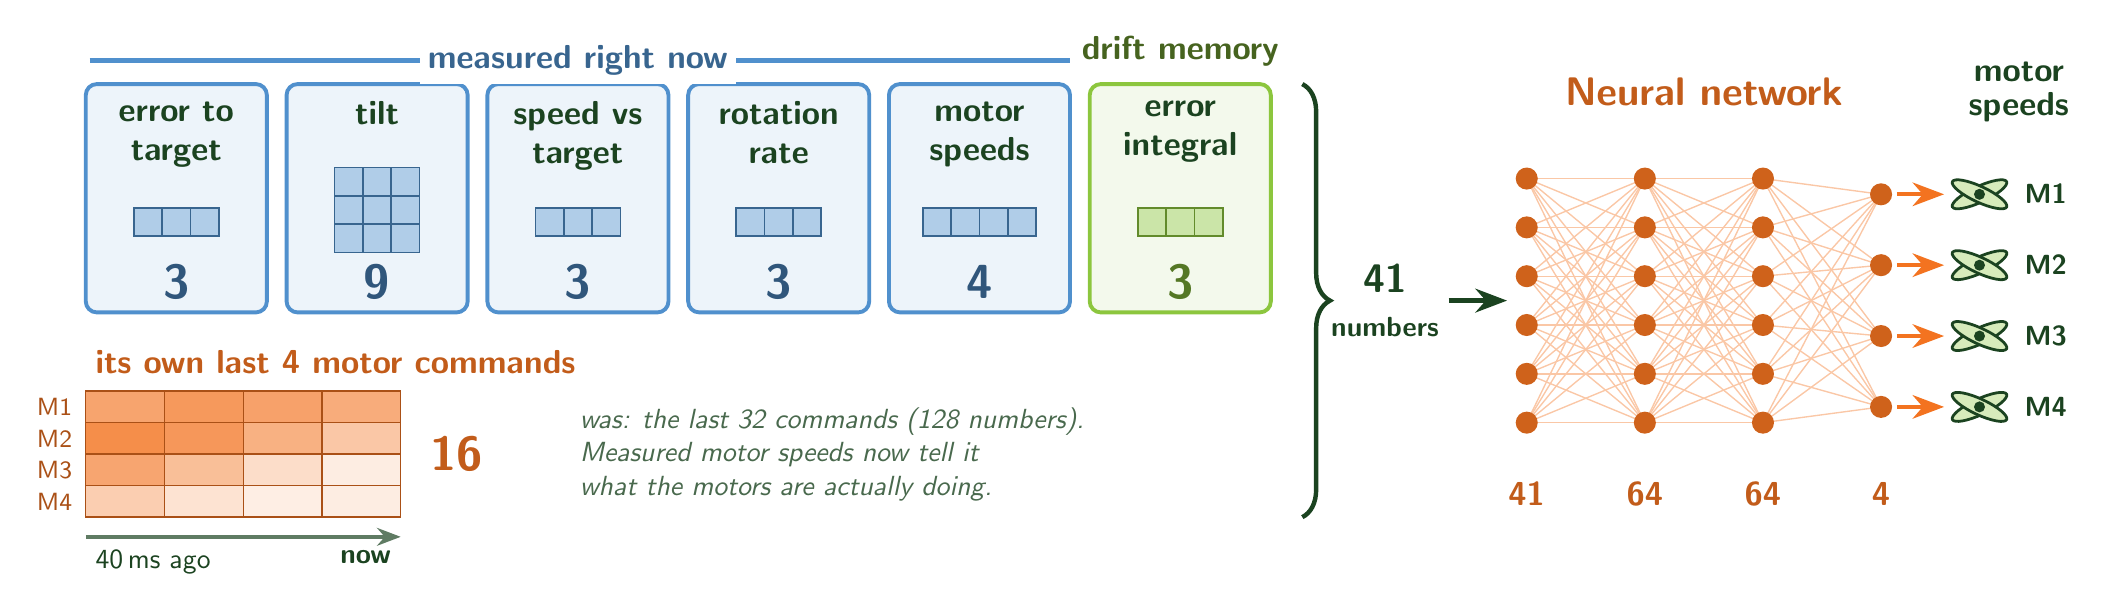
\begin{tikzpicture}
  % ---------- the "right now" groups as cards ----------
  \foreach \x/\ttl/\n/\col in {
      0/{error to\\target}/3/bleu,
      2.55/{tilt}/9/bleu,
      5.1/{speed vs\\target}/3/bleu,
      7.65/{rotation\\rate}/3/bleu,
      10.2/{motor\\speeds}/4/bleu,
      12.75/{error\\integral}/3/vert} {
    \draw[card=\col] (\x-1.15,-1.45) rectangle (\x+1.15,1.45);
    \node[align=center, font=\large\bfseries, text=saclaydk, anchor=north] at (\x,1.35) {\ttl};
    \node[font=\LARGE\bfseries, text=\col!60!black, anchor=south] at (\x,-1.4) {\n};
  }
  % cells inside the cards
  \foreach \x in {0,5.1,7.65} \foreach \i in {-1,0,1}
    \draw[cell=bleu] (\x+\i*\s-\s/2,-0.3-\s/2) rectangle ++(\s,\s);
  \foreach \i in {-1,0,1} \foreach \j in {-1,0,1}
    \draw[cell=bleu] (2.55+\i*\s-\s/2,-0.15+\j*\s-\s/2) rectangle ++(\s,\s);
  \foreach \i in {-1.5,-0.5,0.5,1.5}
    \draw[cell=bleu] (10.2+\i*\s-\s/2,-0.3-\s/2) rectangle ++(\s,\s);
  \foreach \i in {-1,0,1}
    \draw[cell=vert] (12.75+\i*\s-\s/2,-0.3-\s/2) rectangle ++(\s,\s);

  % group headers
  \draw[bleu, line width=1.6pt] (-1.1,1.75) -- (11.35,1.75);
  \node[font=\large\bfseries, text=bleu!70!black, fill=white, inner sep=3pt] at (5.1,1.75) {measured right now};
  \node[font=\large\bfseries, text=vert!50!black, anchor=south] at (12.75,1.55) {drift memory};

  \ifnum\histlen>0
    % ---------- memory: its own last few commands ----------
    \pgfmathtruncatemacro{\nh}{\histlen}
    \pgfmathtruncatemacro{\nnum}{4*\histlen}
    \pgfmathtruncatemacro{\ms}{10*\histlen}
    \def\gw{1.0}
    \node[anchor=south west, font=\large\bfseries, text=mandarine!80!black] at (-1.15,-2.35)
         {its own last \nh\ motor commands};
    \foreach \c in {1,...,\nh} \foreach \r in {0,...,3} {
      \pgfmathtruncatemacro{\v}{max(12, min(85, 45 + 25*sin(\c*23 + \r*70) + 12*sin(\c*61 + \r*20)))}
      \draw[draw=mandarine!70!black, line width=0.5pt, fill=mandarine!\v]
        (-1.15+\c*\gw-\gw, -2.45-\r*0.4) rectangle ++(\gw, -0.4);
    }
    \node[anchor=west, font=\LARGE\bfseries, text=mandarine!80!black] at (-1.15+\nh*\gw+0.25,-3.25) {\nnum};
    \foreach \r/\m in {0/1,1/2,2/3,3/4}
      \node[font=\small, text=mandarine!70!black, anchor=east] at (-1.2,-2.65-\r*0.4) {M\m};
    \draw[-{Stealth[length=3mm]}, line width=1.4pt, saclaydk!70] (-1.15,-4.3) -- (-1.15+\nh*\gw,-4.3);
    \node[anchor=north west, font=\normalsize, text=saclaydk] at (-1.15,-4.35) {\ms\,ms ago};
    \node[anchor=north east, font=\normalsize\bfseries, text=saclaydk] at (-1.15+\nh*\gw,-4.35) {now};
    \node[anchor=west, align=left, font=\normalsize\itshape, text=saclaydk!80] at (5.0,-3.25)
         {was: the last 32 commands (128 numbers).\\Measured motor speeds now tell it\\what the motors are actually doing.};
    \def\ybot{-4.05}
    \def\ny{-1.3}
  \else
    \node[anchor=north west, align=left, font=\normalsize\itshape, text=saclaydk!80] at (-1.15,-1.8)
         {No memory of its own commands (was: the last 32 = 128 numbers).\\
          Measured motor speeds tell it what the motors are actually doing.};
    \def\ybot{-1.45}
    \def\ny{0}
  \fi
  \pgfmathtruncatemacro{\total}{22 + 4*\histlen + 3}

  % ---------- bracket into the network ----------
  \draw[decorate, decoration={brace, amplitude=10pt}, line width=1.6pt, saclaydk]
    (14.3,1.45) -- (14.3,\ybot);
  \node[font=\Large\bfseries, text=saclaydk, align=center] (tot) at (15.35,\ny) {\total\\[-2pt]{\normalsize numbers}};
  \draw[arr, saclaydk] (tot.east) -- (16.9,\ny);

  % ---------- network ----------
  \pgfmathtruncatemacro{\nin}{\histlen > 0 ? 6 : 5}
  \foreach \L/\x/\n/\sp in {0/17.15/\nin/0.62, 1/18.65/6/0.62, 2/20.15/6/0.62, 3/21.65/4/0.9} {
    \foreach \k in {1,...,\n} \coordinate (N\L-\k) at (\x, {\ny + (\n+1)/2*\sp - \k*\sp});
  }
  \foreach \a/\na/\b/\nb in {0/\nin/1/6, 1/6/2/6, 2/6/3/4}
    \foreach \i in {1,...,\na} \foreach \j in {1,...,\nb}
      \draw[mandarine!40, line width=0.5pt] (N\a-\i) -- (N\b-\j);
  \foreach \L/\n in {0/\nin,1/6,2/6,3/4} \foreach \k in {1,...,\n}
    \fill[mandarine!85!black] (N\L-\k) circle (0.14);
  \foreach \x/\lab in {17.15/\total, 18.65/64, 20.15/64, 21.65/4}
    \node[font=\large\bfseries, text=mandarine!80!black] at (\x,\ny-2.45) {\lab};
  \node[font=\Large\bfseries, text=mandarine!80!black] at (19.4,\ny+2.65) {Neural network};

  % ---------- outputs: 4 propellers ----------
  \foreach \k in {1,...,4} {
    \coordinate (P) at ($(N3-\k)+(1.25,0)$);
    \draw[arr, mandarine, line width=1.4pt] ($(N3-\k)+(0.2,0)$) -- ($(P)+(-0.45,0)$);
    \draw[saclaydk, fill=vert!35, line width=1pt, rotate around={25:(P)}] (P) ellipse (0.38 and 0.1);
    \draw[saclaydk, fill=vert!35, line width=1pt, rotate around={-25:(P)}] (P) ellipse (0.38 and 0.1);
    \fill[saclaydk] (P) circle (0.07);
    \node[anchor=west, font=\normalsize\bfseries, text=saclaydk] at ($(P)+(0.45,0)$) {M\k};
  }
  \node[align=center, font=\large\bfseries, text=saclaydk] at (23.4,\ny+2.65) {motor\\[-2pt]speeds};
\end{tikzpicture}
\end{document}
"   (25 inputs)
% Compiled on its own it gives the 4-step version. In the poster:
%   \includegraphics[width=\linewidth]{images/fig_inputs_short_poster.pdf}
\documentclass[12pt, border=4pt]{standalone}
\usepackage{tikz}
\usetikzlibrary{arrows.meta,positioning,calc,decorations.pathreplacing}
\renewcommand{\familydefault}{\sfdefault}

\definecolor{saclaydk}{RGB}{27,67,32}
\definecolor{mandarine}{RGB}{243,115,32}
\definecolor{vert}{RGB}{140,198,62}
\definecolor{bleu}{RGB}{80,144,205}
\definecolor{rouge}{RGB}{198,11,70}

\tikzset{
  cell/.style={draw=#1!70!black, fill=#1!45, line width=0.6pt},
  card/.style={draw=#1, fill=#1!10, rounded corners=4pt, line width=1.4pt},
  arr/.style={-{Stealth[length=4mm,width=3mm]}, line width=2pt},
}
\newcommand{\s}{0.36} % cell size
\providecommand{\histlen}{4}

\begin{document}
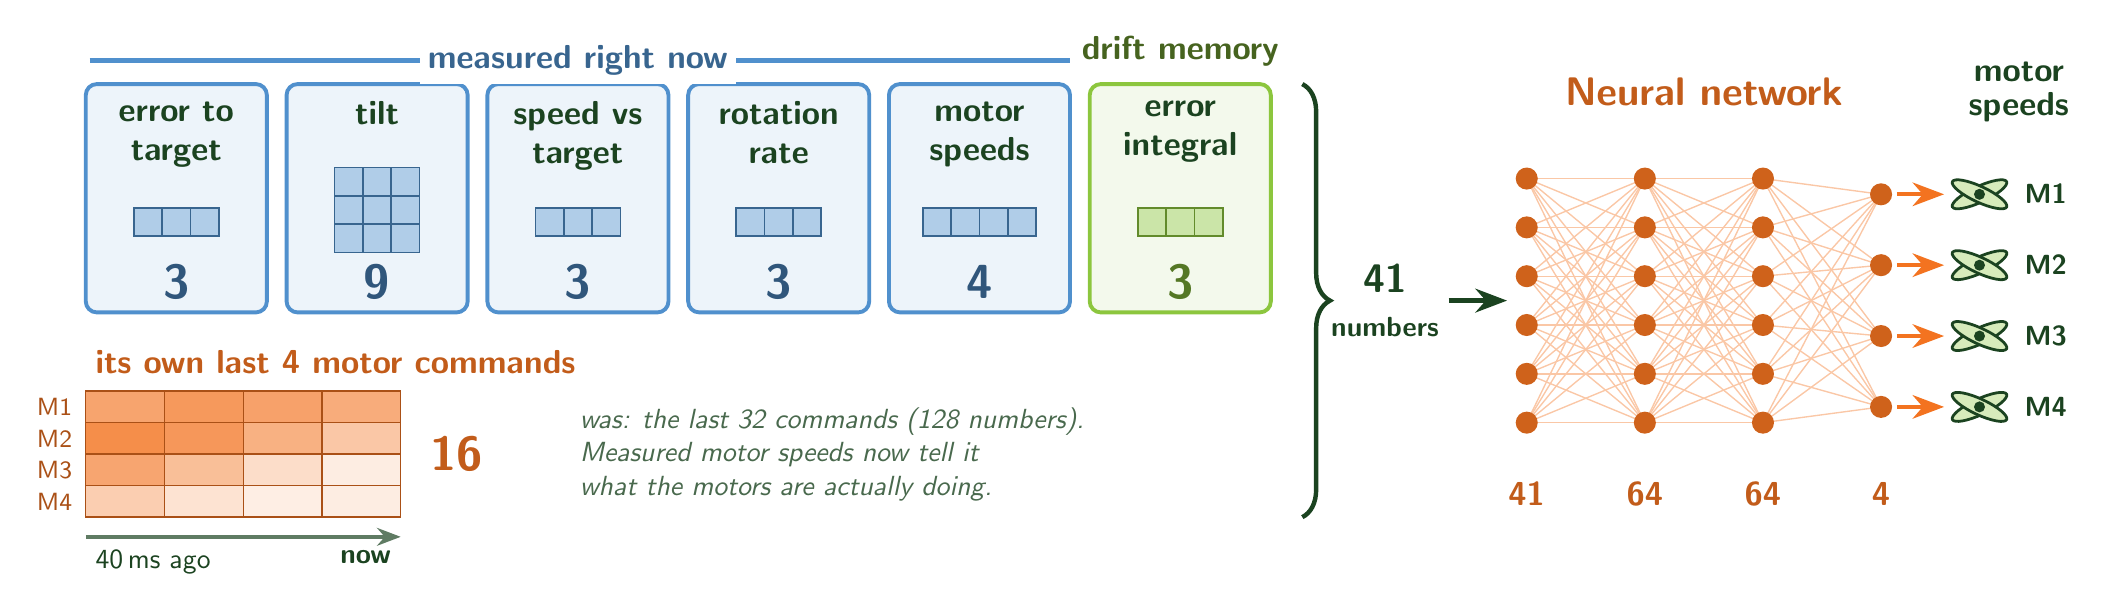
\begin{tikzpicture}
  % ---------- the "right now" groups as cards ----------
  \foreach \x/\ttl/\n/\col in {
      0/{error to\\target}/3/bleu,
      2.55/{tilt}/9/bleu,
      5.1/{speed vs\\target}/3/bleu,
      7.65/{rotation\\rate}/3/bleu,
      10.2/{motor\\speeds}/4/bleu,
      12.75/{error\\integral}/3/vert} {
    \draw[card=\col] (\x-1.15,-1.45) rectangle (\x+1.15,1.45);
    \node[align=center, font=\large\bfseries, text=saclaydk, anchor=north] at (\x,1.35) {\ttl};
    \node[font=\LARGE\bfseries, text=\col!60!black, anchor=south] at (\x,-1.4) {\n};
  }
  % cells inside the cards
  \foreach \x in {0,5.1,7.65} \foreach \i in {-1,0,1}
    \draw[cell=bleu] (\x+\i*\s-\s/2,-0.3-\s/2) rectangle ++(\s,\s);
  \foreach \i in {-1,0,1} \foreach \j in {-1,0,1}
    \draw[cell=bleu] (2.55+\i*\s-\s/2,-0.15+\j*\s-\s/2) rectangle ++(\s,\s);
  \foreach \i in {-1.5,-0.5,0.5,1.5}
    \draw[cell=bleu] (10.2+\i*\s-\s/2,-0.3-\s/2) rectangle ++(\s,\s);
  \foreach \i in {-1,0,1}
    \draw[cell=vert] (12.75+\i*\s-\s/2,-0.3-\s/2) rectangle ++(\s,\s);

  % group headers
  \draw[bleu, line width=1.6pt] (-1.1,1.75) -- (11.35,1.75);
  \node[font=\large\bfseries, text=bleu!70!black, fill=white, inner sep=3pt] at (5.1,1.75) {measured right now};
  \node[font=\large\bfseries, text=vert!50!black, anchor=south] at (12.75,1.55) {drift memory};

  \ifnum\histlen>0
    % ---------- memory: its own last few commands ----------
    \pgfmathtruncatemacro{\nh}{\histlen}
    \pgfmathtruncatemacro{\nnum}{4*\histlen}
    \pgfmathtruncatemacro{\ms}{10*\histlen}
    \def\gw{1.0}
    \node[anchor=south west, font=\large\bfseries, text=mandarine!80!black] at (-1.15,-2.35)
         {its own last \nh\ motor commands};
    \foreach \c in {1,...,\nh} \foreach \r in {0,...,3} {
      \pgfmathtruncatemacro{\v}{max(12, min(85, 45 + 25*sin(\c*23 + \r*70) + 12*sin(\c*61 + \r*20)))}
      \draw[draw=mandarine!70!black, line width=0.5pt, fill=mandarine!\v]
        (-1.15+\c*\gw-\gw, -2.45-\r*0.4) rectangle ++(\gw, -0.4);
    }
    \node[anchor=west, font=\LARGE\bfseries, text=mandarine!80!black] at (-1.15+\nh*\gw+0.25,-3.25) {\nnum};
    \foreach \r/\m in {0/1,1/2,2/3,3/4}
      \node[font=\small, text=mandarine!70!black, anchor=east] at (-1.2,-2.65-\r*0.4) {M\m};
    \draw[-{Stealth[length=3mm]}, line width=1.4pt, saclaydk!70] (-1.15,-4.3) -- (-1.15+\nh*\gw,-4.3);
    \node[anchor=north west, font=\normalsize, text=saclaydk] at (-1.15,-4.35) {\ms\,ms ago};
    \node[anchor=north east, font=\normalsize\bfseries, text=saclaydk] at (-1.15+\nh*\gw,-4.35) {now};
    \node[anchor=west, align=left, font=\normalsize\itshape, text=saclaydk!80] at (5.0,-3.25)
         {was: the last 32 commands (128 numbers).\\Measured motor speeds now tell it\\what the motors are actually doing.};
    \def\ybot{-4.05}
    \def\ny{-1.3}
  \else
    \node[anchor=north west, align=left, font=\normalsize\itshape, text=saclaydk!80] at (-1.15,-1.8)
         {No memory of its own commands (was: the last 32 = 128 numbers).\\
          Measured motor speeds tell it what the motors are actually doing.};
    \def\ybot{-1.45}
    \def\ny{0}
  \fi
  \pgfmathtruncatemacro{\total}{22 + 4*\histlen + 3}

  % ---------- bracket into the network ----------
  \draw[decorate, decoration={brace, amplitude=10pt}, line width=1.6pt, saclaydk]
    (14.3,1.45) -- (14.3,\ybot);
  \node[font=\Large\bfseries, text=saclaydk, align=center] (tot) at (15.35,\ny) {\total\\[-2pt]{\normalsize numbers}};
  \draw[arr, saclaydk] (tot.east) -- (16.9,\ny);

  % ---------- network ----------
  \pgfmathtruncatemacro{\nin}{\histlen > 0 ? 6 : 5}
  \foreach \L/\x/\n/\sp in {0/17.15/\nin/0.62, 1/18.65/6/0.62, 2/20.15/6/0.62, 3/21.65/4/0.9} {
    \foreach \k in {1,...,\n} \coordinate (N\L-\k) at (\x, {\ny + (\n+1)/2*\sp - \k*\sp});
  }
  \foreach \a/\na/\b/\nb in {0/\nin/1/6, 1/6/2/6, 2/6/3/4}
    \foreach \i in {1,...,\na} \foreach \j in {1,...,\nb}
      \draw[mandarine!40, line width=0.5pt] (N\a-\i) -- (N\b-\j);
  \foreach \L/\n in {0/\nin,1/6,2/6,3/4} \foreach \k in {1,...,\n}
    \fill[mandarine!85!black] (N\L-\k) circle (0.14);
  \foreach \x/\lab in {17.15/\total, 18.65/64, 20.15/64, 21.65/4}
    \node[font=\large\bfseries, text=mandarine!80!black] at (\x,\ny-2.45) {\lab};
  \node[font=\Large\bfseries, text=mandarine!80!black] at (19.4,\ny+2.65) {Neural network};

  % ---------- outputs: 4 propellers ----------
  \foreach \k in {1,...,4} {
    \coordinate (P) at ($(N3-\k)+(1.25,0)$);
    \draw[arr, mandarine, line width=1.4pt] ($(N3-\k)+(0.2,0)$) -- ($(P)+(-0.45,0)$);
    \draw[saclaydk, fill=vert!35, line width=1pt, rotate around={25:(P)}] (P) ellipse (0.38 and 0.1);
    \draw[saclaydk, fill=vert!35, line width=1pt, rotate around={-25:(P)}] (P) ellipse (0.38 and 0.1);
    \fill[saclaydk] (P) circle (0.07);
    \node[anchor=west, font=\normalsize\bfseries, text=saclaydk] at ($(P)+(0.45,0)$) {M\k};
  }
  \node[align=center, font=\large\bfseries, text=saclaydk] at (23.4,\ny+2.65) {motor\\[-2pt]speeds};
\end{tikzpicture}
\end{document}
"   (41 inputs)
%   pdflatex -jobname=fig_inputs_none_poster  "\def\histlen{0}% "What the network sees" with measured motor speeds, for the A1 poster.
% One source, two figures (set \histlen before \input):
%   pdflatex -jobname=fig_inputs_short_poster "\def\histlen{4}% "What the network sees" with measured motor speeds, for the A1 poster.
% One source, two figures (set \histlen before \input):
%   pdflatex -jobname=fig_inputs_short_poster "\def\histlen{4}\input{fig_inputs_rpm_poster.tex}"   (41 inputs)
%   pdflatex -jobname=fig_inputs_none_poster  "\def\histlen{0}\input{fig_inputs_rpm_poster.tex}"   (25 inputs)
% Compiled on its own it gives the 4-step version. In the poster:
%   \includegraphics[width=\linewidth]{images/fig_inputs_short_poster.pdf}
\documentclass[12pt, border=4pt]{standalone}
\usepackage{tikz}
\usetikzlibrary{arrows.meta,positioning,calc,decorations.pathreplacing}
\renewcommand{\familydefault}{\sfdefault}

\definecolor{saclaydk}{RGB}{27,67,32}
\definecolor{mandarine}{RGB}{243,115,32}
\definecolor{vert}{RGB}{140,198,62}
\definecolor{bleu}{RGB}{80,144,205}
\definecolor{rouge}{RGB}{198,11,70}

\tikzset{
  cell/.style={draw=#1!70!black, fill=#1!45, line width=0.6pt},
  card/.style={draw=#1, fill=#1!10, rounded corners=4pt, line width=1.4pt},
  arr/.style={-{Stealth[length=4mm,width=3mm]}, line width=2pt},
}
\newcommand{\s}{0.36} % cell size
\providecommand{\histlen}{4}

\begin{document}
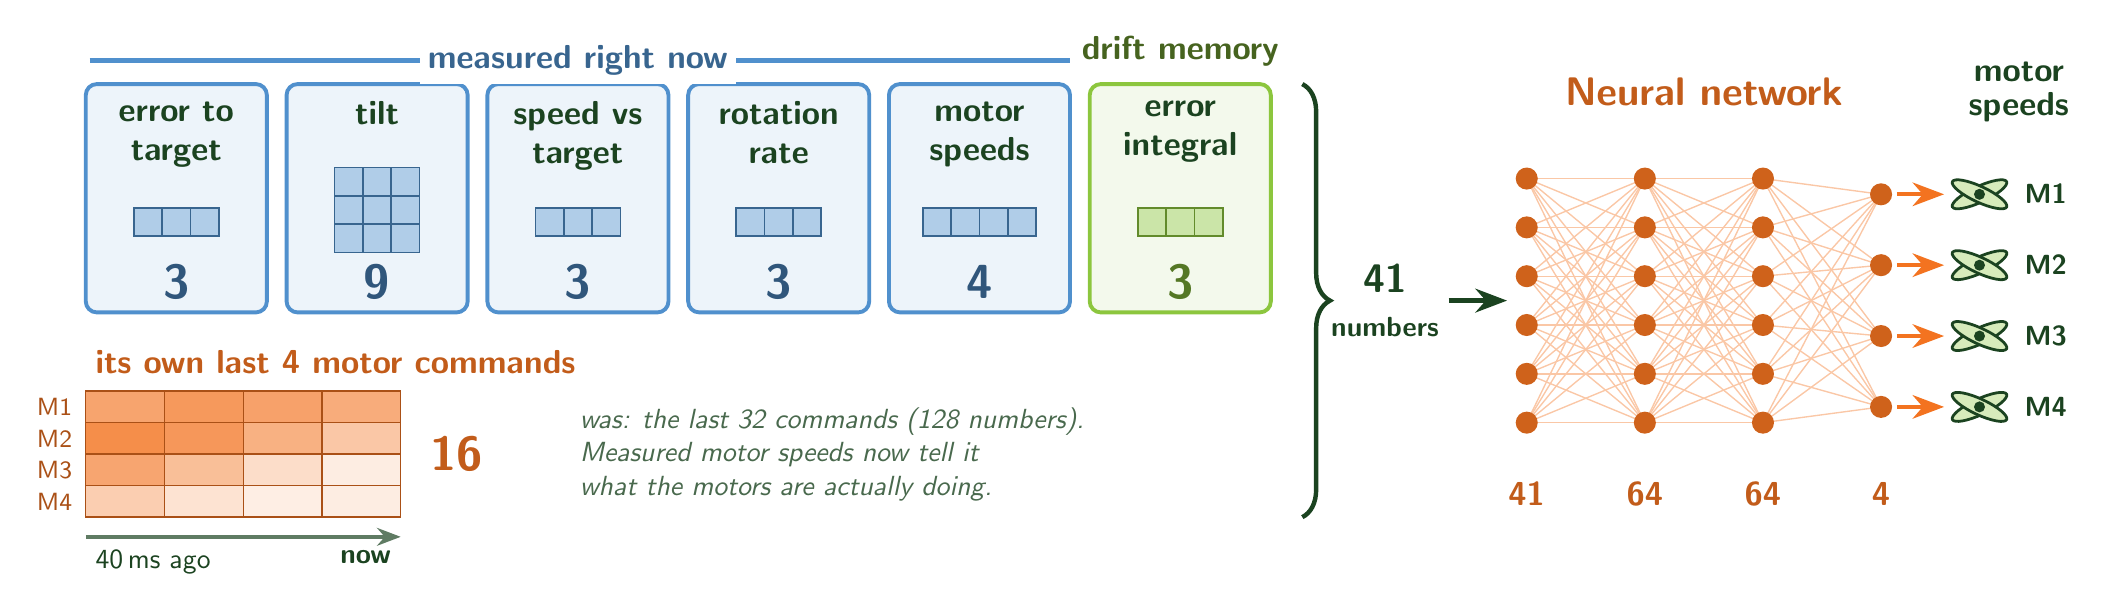
\begin{tikzpicture}
  % ---------- the "right now" groups as cards ----------
  \foreach \x/\ttl/\n/\col in {
      0/{error to\\target}/3/bleu,
      2.55/{tilt}/9/bleu,
      5.1/{speed vs\\target}/3/bleu,
      7.65/{rotation\\rate}/3/bleu,
      10.2/{motor\\speeds}/4/bleu,
      12.75/{error\\integral}/3/vert} {
    \draw[card=\col] (\x-1.15,-1.45) rectangle (\x+1.15,1.45);
    \node[align=center, font=\large\bfseries, text=saclaydk, anchor=north] at (\x,1.35) {\ttl};
    \node[font=\LARGE\bfseries, text=\col!60!black, anchor=south] at (\x,-1.4) {\n};
  }
  % cells inside the cards
  \foreach \x in {0,5.1,7.65} \foreach \i in {-1,0,1}
    \draw[cell=bleu] (\x+\i*\s-\s/2,-0.3-\s/2) rectangle ++(\s,\s);
  \foreach \i in {-1,0,1} \foreach \j in {-1,0,1}
    \draw[cell=bleu] (2.55+\i*\s-\s/2,-0.15+\j*\s-\s/2) rectangle ++(\s,\s);
  \foreach \i in {-1.5,-0.5,0.5,1.5}
    \draw[cell=bleu] (10.2+\i*\s-\s/2,-0.3-\s/2) rectangle ++(\s,\s);
  \foreach \i in {-1,0,1}
    \draw[cell=vert] (12.75+\i*\s-\s/2,-0.3-\s/2) rectangle ++(\s,\s);

  % group headers
  \draw[bleu, line width=1.6pt] (-1.1,1.75) -- (11.35,1.75);
  \node[font=\large\bfseries, text=bleu!70!black, fill=white, inner sep=3pt] at (5.1,1.75) {measured right now};
  \node[font=\large\bfseries, text=vert!50!black, anchor=south] at (12.75,1.55) {drift memory};

  \ifnum\histlen>0
    % ---------- memory: its own last few commands ----------
    \pgfmathtruncatemacro{\nh}{\histlen}
    \pgfmathtruncatemacro{\nnum}{4*\histlen}
    \pgfmathtruncatemacro{\ms}{10*\histlen}
    \def\gw{1.0}
    \node[anchor=south west, font=\large\bfseries, text=mandarine!80!black] at (-1.15,-2.35)
         {its own last \nh\ motor commands};
    \foreach \c in {1,...,\nh} \foreach \r in {0,...,3} {
      \pgfmathtruncatemacro{\v}{max(12, min(85, 45 + 25*sin(\c*23 + \r*70) + 12*sin(\c*61 + \r*20)))}
      \draw[draw=mandarine!70!black, line width=0.5pt, fill=mandarine!\v]
        (-1.15+\c*\gw-\gw, -2.45-\r*0.4) rectangle ++(\gw, -0.4);
    }
    \node[anchor=west, font=\LARGE\bfseries, text=mandarine!80!black] at (-1.15+\nh*\gw+0.25,-3.25) {\nnum};
    \foreach \r/\m in {0/1,1/2,2/3,3/4}
      \node[font=\small, text=mandarine!70!black, anchor=east] at (-1.2,-2.65-\r*0.4) {M\m};
    \draw[-{Stealth[length=3mm]}, line width=1.4pt, saclaydk!70] (-1.15,-4.3) -- (-1.15+\nh*\gw,-4.3);
    \node[anchor=north west, font=\normalsize, text=saclaydk] at (-1.15,-4.35) {\ms\,ms ago};
    \node[anchor=north east, font=\normalsize\bfseries, text=saclaydk] at (-1.15+\nh*\gw,-4.35) {now};
    \node[anchor=west, align=left, font=\normalsize\itshape, text=saclaydk!80] at (5.0,-3.25)
         {was: the last 32 commands (128 numbers).\\Measured motor speeds now tell it\\what the motors are actually doing.};
    \def\ybot{-4.05}
    \def\ny{-1.3}
  \else
    \node[anchor=north west, align=left, font=\normalsize\itshape, text=saclaydk!80] at (-1.15,-1.8)
         {No memory of its own commands (was: the last 32 = 128 numbers).\\
          Measured motor speeds tell it what the motors are actually doing.};
    \def\ybot{-1.45}
    \def\ny{0}
  \fi
  \pgfmathtruncatemacro{\total}{22 + 4*\histlen + 3}

  % ---------- bracket into the network ----------
  \draw[decorate, decoration={brace, amplitude=10pt}, line width=1.6pt, saclaydk]
    (14.3,1.45) -- (14.3,\ybot);
  \node[font=\Large\bfseries, text=saclaydk, align=center] (tot) at (15.35,\ny) {\total\\[-2pt]{\normalsize numbers}};
  \draw[arr, saclaydk] (tot.east) -- (16.9,\ny);

  % ---------- network ----------
  \pgfmathtruncatemacro{\nin}{\histlen > 0 ? 6 : 5}
  \foreach \L/\x/\n/\sp in {0/17.15/\nin/0.62, 1/18.65/6/0.62, 2/20.15/6/0.62, 3/21.65/4/0.9} {
    \foreach \k in {1,...,\n} \coordinate (N\L-\k) at (\x, {\ny + (\n+1)/2*\sp - \k*\sp});
  }
  \foreach \a/\na/\b/\nb in {0/\nin/1/6, 1/6/2/6, 2/6/3/4}
    \foreach \i in {1,...,\na} \foreach \j in {1,...,\nb}
      \draw[mandarine!40, line width=0.5pt] (N\a-\i) -- (N\b-\j);
  \foreach \L/\n in {0/\nin,1/6,2/6,3/4} \foreach \k in {1,...,\n}
    \fill[mandarine!85!black] (N\L-\k) circle (0.14);
  \foreach \x/\lab in {17.15/\total, 18.65/64, 20.15/64, 21.65/4}
    \node[font=\large\bfseries, text=mandarine!80!black] at (\x,\ny-2.45) {\lab};
  \node[font=\Large\bfseries, text=mandarine!80!black] at (19.4,\ny+2.65) {Neural network};

  % ---------- outputs: 4 propellers ----------
  \foreach \k in {1,...,4} {
    \coordinate (P) at ($(N3-\k)+(1.25,0)$);
    \draw[arr, mandarine, line width=1.4pt] ($(N3-\k)+(0.2,0)$) -- ($(P)+(-0.45,0)$);
    \draw[saclaydk, fill=vert!35, line width=1pt, rotate around={25:(P)}] (P) ellipse (0.38 and 0.1);
    \draw[saclaydk, fill=vert!35, line width=1pt, rotate around={-25:(P)}] (P) ellipse (0.38 and 0.1);
    \fill[saclaydk] (P) circle (0.07);
    \node[anchor=west, font=\normalsize\bfseries, text=saclaydk] at ($(P)+(0.45,0)$) {M\k};
  }
  \node[align=center, font=\large\bfseries, text=saclaydk] at (23.4,\ny+2.65) {motor\\[-2pt]speeds};
\end{tikzpicture}
\end{document}
"   (41 inputs)
%   pdflatex -jobname=fig_inputs_none_poster  "\def\histlen{0}% "What the network sees" with measured motor speeds, for the A1 poster.
% One source, two figures (set \histlen before \input):
%   pdflatex -jobname=fig_inputs_short_poster "\def\histlen{4}\input{fig_inputs_rpm_poster.tex}"   (41 inputs)
%   pdflatex -jobname=fig_inputs_none_poster  "\def\histlen{0}\input{fig_inputs_rpm_poster.tex}"   (25 inputs)
% Compiled on its own it gives the 4-step version. In the poster:
%   \includegraphics[width=\linewidth]{images/fig_inputs_short_poster.pdf}
\documentclass[12pt, border=4pt]{standalone}
\usepackage{tikz}
\usetikzlibrary{arrows.meta,positioning,calc,decorations.pathreplacing}
\renewcommand{\familydefault}{\sfdefault}

\definecolor{saclaydk}{RGB}{27,67,32}
\definecolor{mandarine}{RGB}{243,115,32}
\definecolor{vert}{RGB}{140,198,62}
\definecolor{bleu}{RGB}{80,144,205}
\definecolor{rouge}{RGB}{198,11,70}

\tikzset{
  cell/.style={draw=#1!70!black, fill=#1!45, line width=0.6pt},
  card/.style={draw=#1, fill=#1!10, rounded corners=4pt, line width=1.4pt},
  arr/.style={-{Stealth[length=4mm,width=3mm]}, line width=2pt},
}
\newcommand{\s}{0.36} % cell size
\providecommand{\histlen}{4}

\begin{document}
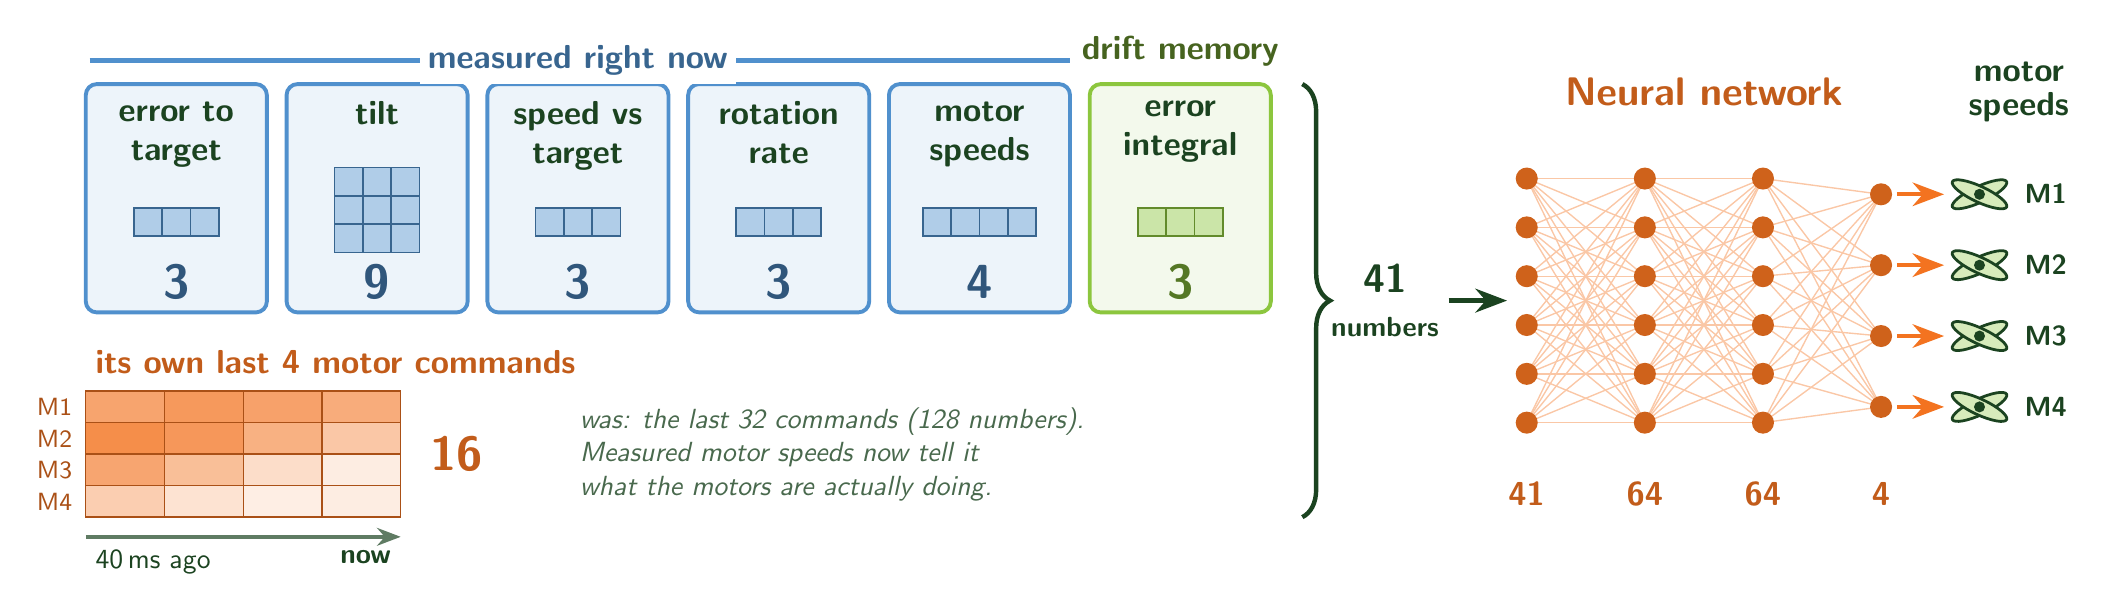
\begin{tikzpicture}
  % ---------- the "right now" groups as cards ----------
  \foreach \x/\ttl/\n/\col in {
      0/{error to\\target}/3/bleu,
      2.55/{tilt}/9/bleu,
      5.1/{speed vs\\target}/3/bleu,
      7.65/{rotation\\rate}/3/bleu,
      10.2/{motor\\speeds}/4/bleu,
      12.75/{error\\integral}/3/vert} {
    \draw[card=\col] (\x-1.15,-1.45) rectangle (\x+1.15,1.45);
    \node[align=center, font=\large\bfseries, text=saclaydk, anchor=north] at (\x,1.35) {\ttl};
    \node[font=\LARGE\bfseries, text=\col!60!black, anchor=south] at (\x,-1.4) {\n};
  }
  % cells inside the cards
  \foreach \x in {0,5.1,7.65} \foreach \i in {-1,0,1}
    \draw[cell=bleu] (\x+\i*\s-\s/2,-0.3-\s/2) rectangle ++(\s,\s);
  \foreach \i in {-1,0,1} \foreach \j in {-1,0,1}
    \draw[cell=bleu] (2.55+\i*\s-\s/2,-0.15+\j*\s-\s/2) rectangle ++(\s,\s);
  \foreach \i in {-1.5,-0.5,0.5,1.5}
    \draw[cell=bleu] (10.2+\i*\s-\s/2,-0.3-\s/2) rectangle ++(\s,\s);
  \foreach \i in {-1,0,1}
    \draw[cell=vert] (12.75+\i*\s-\s/2,-0.3-\s/2) rectangle ++(\s,\s);

  % group headers
  \draw[bleu, line width=1.6pt] (-1.1,1.75) -- (11.35,1.75);
  \node[font=\large\bfseries, text=bleu!70!black, fill=white, inner sep=3pt] at (5.1,1.75) {measured right now};
  \node[font=\large\bfseries, text=vert!50!black, anchor=south] at (12.75,1.55) {drift memory};

  \ifnum\histlen>0
    % ---------- memory: its own last few commands ----------
    \pgfmathtruncatemacro{\nh}{\histlen}
    \pgfmathtruncatemacro{\nnum}{4*\histlen}
    \pgfmathtruncatemacro{\ms}{10*\histlen}
    \def\gw{1.0}
    \node[anchor=south west, font=\large\bfseries, text=mandarine!80!black] at (-1.15,-2.35)
         {its own last \nh\ motor commands};
    \foreach \c in {1,...,\nh} \foreach \r in {0,...,3} {
      \pgfmathtruncatemacro{\v}{max(12, min(85, 45 + 25*sin(\c*23 + \r*70) + 12*sin(\c*61 + \r*20)))}
      \draw[draw=mandarine!70!black, line width=0.5pt, fill=mandarine!\v]
        (-1.15+\c*\gw-\gw, -2.45-\r*0.4) rectangle ++(\gw, -0.4);
    }
    \node[anchor=west, font=\LARGE\bfseries, text=mandarine!80!black] at (-1.15+\nh*\gw+0.25,-3.25) {\nnum};
    \foreach \r/\m in {0/1,1/2,2/3,3/4}
      \node[font=\small, text=mandarine!70!black, anchor=east] at (-1.2,-2.65-\r*0.4) {M\m};
    \draw[-{Stealth[length=3mm]}, line width=1.4pt, saclaydk!70] (-1.15,-4.3) -- (-1.15+\nh*\gw,-4.3);
    \node[anchor=north west, font=\normalsize, text=saclaydk] at (-1.15,-4.35) {\ms\,ms ago};
    \node[anchor=north east, font=\normalsize\bfseries, text=saclaydk] at (-1.15+\nh*\gw,-4.35) {now};
    \node[anchor=west, align=left, font=\normalsize\itshape, text=saclaydk!80] at (5.0,-3.25)
         {was: the last 32 commands (128 numbers).\\Measured motor speeds now tell it\\what the motors are actually doing.};
    \def\ybot{-4.05}
    \def\ny{-1.3}
  \else
    \node[anchor=north west, align=left, font=\normalsize\itshape, text=saclaydk!80] at (-1.15,-1.8)
         {No memory of its own commands (was: the last 32 = 128 numbers).\\
          Measured motor speeds tell it what the motors are actually doing.};
    \def\ybot{-1.45}
    \def\ny{0}
  \fi
  \pgfmathtruncatemacro{\total}{22 + 4*\histlen + 3}

  % ---------- bracket into the network ----------
  \draw[decorate, decoration={brace, amplitude=10pt}, line width=1.6pt, saclaydk]
    (14.3,1.45) -- (14.3,\ybot);
  \node[font=\Large\bfseries, text=saclaydk, align=center] (tot) at (15.35,\ny) {\total\\[-2pt]{\normalsize numbers}};
  \draw[arr, saclaydk] (tot.east) -- (16.9,\ny);

  % ---------- network ----------
  \pgfmathtruncatemacro{\nin}{\histlen > 0 ? 6 : 5}
  \foreach \L/\x/\n/\sp in {0/17.15/\nin/0.62, 1/18.65/6/0.62, 2/20.15/6/0.62, 3/21.65/4/0.9} {
    \foreach \k in {1,...,\n} \coordinate (N\L-\k) at (\x, {\ny + (\n+1)/2*\sp - \k*\sp});
  }
  \foreach \a/\na/\b/\nb in {0/\nin/1/6, 1/6/2/6, 2/6/3/4}
    \foreach \i in {1,...,\na} \foreach \j in {1,...,\nb}
      \draw[mandarine!40, line width=0.5pt] (N\a-\i) -- (N\b-\j);
  \foreach \L/\n in {0/\nin,1/6,2/6,3/4} \foreach \k in {1,...,\n}
    \fill[mandarine!85!black] (N\L-\k) circle (0.14);
  \foreach \x/\lab in {17.15/\total, 18.65/64, 20.15/64, 21.65/4}
    \node[font=\large\bfseries, text=mandarine!80!black] at (\x,\ny-2.45) {\lab};
  \node[font=\Large\bfseries, text=mandarine!80!black] at (19.4,\ny+2.65) {Neural network};

  % ---------- outputs: 4 propellers ----------
  \foreach \k in {1,...,4} {
    \coordinate (P) at ($(N3-\k)+(1.25,0)$);
    \draw[arr, mandarine, line width=1.4pt] ($(N3-\k)+(0.2,0)$) -- ($(P)+(-0.45,0)$);
    \draw[saclaydk, fill=vert!35, line width=1pt, rotate around={25:(P)}] (P) ellipse (0.38 and 0.1);
    \draw[saclaydk, fill=vert!35, line width=1pt, rotate around={-25:(P)}] (P) ellipse (0.38 and 0.1);
    \fill[saclaydk] (P) circle (0.07);
    \node[anchor=west, font=\normalsize\bfseries, text=saclaydk] at ($(P)+(0.45,0)$) {M\k};
  }
  \node[align=center, font=\large\bfseries, text=saclaydk] at (23.4,\ny+2.65) {motor\\[-2pt]speeds};
\end{tikzpicture}
\end{document}
"   (25 inputs)
% Compiled on its own it gives the 4-step version. In the poster:
%   \includegraphics[width=\linewidth]{images/fig_inputs_short_poster.pdf}
\documentclass[12pt, border=4pt]{standalone}
\usepackage{tikz}
\usetikzlibrary{arrows.meta,positioning,calc,decorations.pathreplacing}
\renewcommand{\familydefault}{\sfdefault}

\definecolor{saclaydk}{RGB}{27,67,32}
\definecolor{mandarine}{RGB}{243,115,32}
\definecolor{vert}{RGB}{140,198,62}
\definecolor{bleu}{RGB}{80,144,205}
\definecolor{rouge}{RGB}{198,11,70}

\tikzset{
  cell/.style={draw=#1!70!black, fill=#1!45, line width=0.6pt},
  card/.style={draw=#1, fill=#1!10, rounded corners=4pt, line width=1.4pt},
  arr/.style={-{Stealth[length=4mm,width=3mm]}, line width=2pt},
}
\newcommand{\s}{0.36} % cell size
\providecommand{\histlen}{4}

\begin{document}
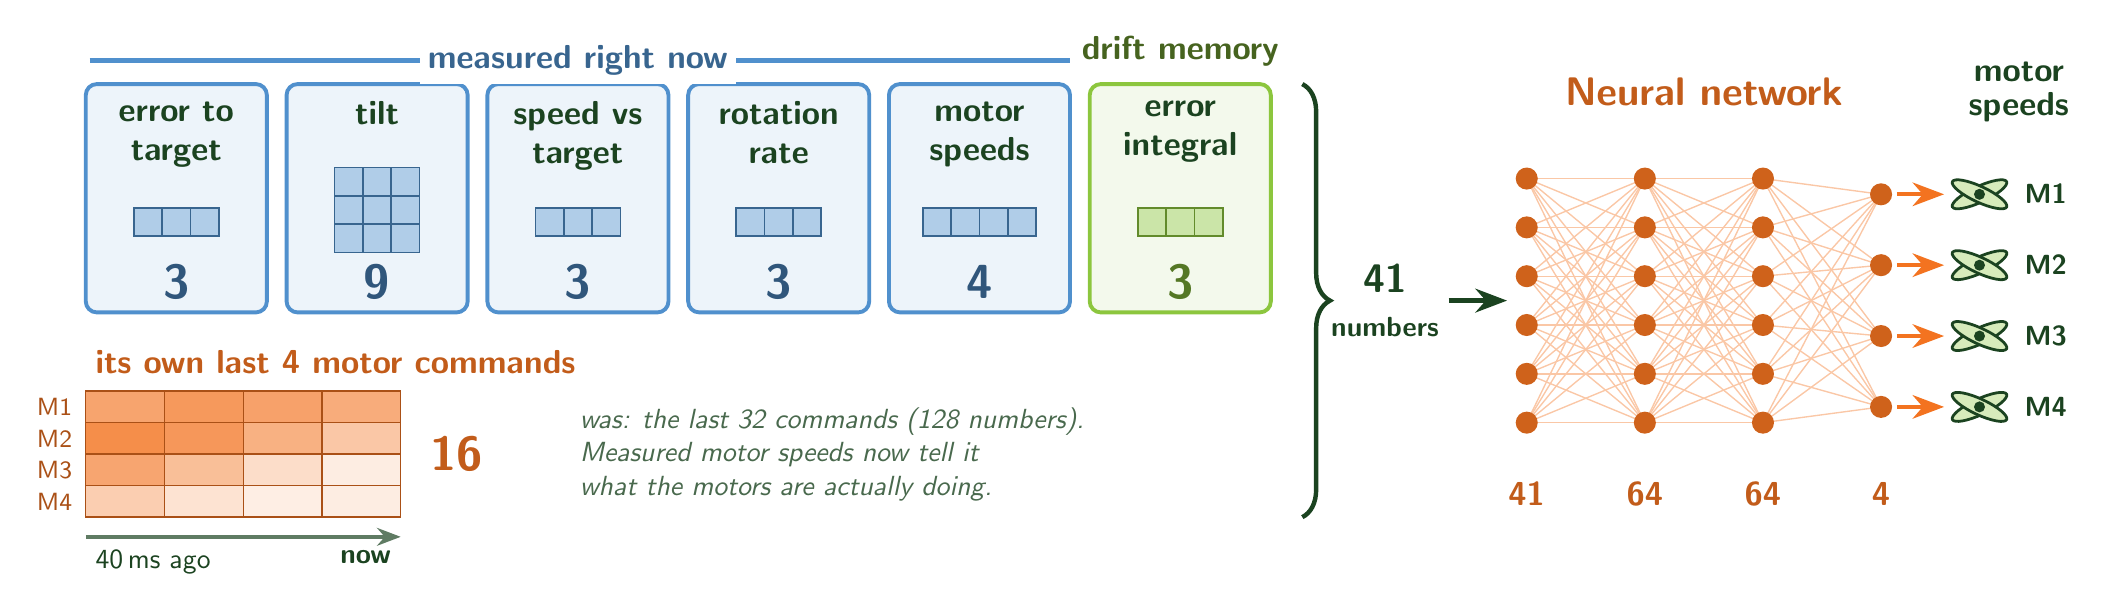
\begin{tikzpicture}
  % ---------- the "right now" groups as cards ----------
  \foreach \x/\ttl/\n/\col in {
      0/{error to\\target}/3/bleu,
      2.55/{tilt}/9/bleu,
      5.1/{speed vs\\target}/3/bleu,
      7.65/{rotation\\rate}/3/bleu,
      10.2/{motor\\speeds}/4/bleu,
      12.75/{error\\integral}/3/vert} {
    \draw[card=\col] (\x-1.15,-1.45) rectangle (\x+1.15,1.45);
    \node[align=center, font=\large\bfseries, text=saclaydk, anchor=north] at (\x,1.35) {\ttl};
    \node[font=\LARGE\bfseries, text=\col!60!black, anchor=south] at (\x,-1.4) {\n};
  }
  % cells inside the cards
  \foreach \x in {0,5.1,7.65} \foreach \i in {-1,0,1}
    \draw[cell=bleu] (\x+\i*\s-\s/2,-0.3-\s/2) rectangle ++(\s,\s);
  \foreach \i in {-1,0,1} \foreach \j in {-1,0,1}
    \draw[cell=bleu] (2.55+\i*\s-\s/2,-0.15+\j*\s-\s/2) rectangle ++(\s,\s);
  \foreach \i in {-1.5,-0.5,0.5,1.5}
    \draw[cell=bleu] (10.2+\i*\s-\s/2,-0.3-\s/2) rectangle ++(\s,\s);
  \foreach \i in {-1,0,1}
    \draw[cell=vert] (12.75+\i*\s-\s/2,-0.3-\s/2) rectangle ++(\s,\s);

  % group headers
  \draw[bleu, line width=1.6pt] (-1.1,1.75) -- (11.35,1.75);
  \node[font=\large\bfseries, text=bleu!70!black, fill=white, inner sep=3pt] at (5.1,1.75) {measured right now};
  \node[font=\large\bfseries, text=vert!50!black, anchor=south] at (12.75,1.55) {drift memory};

  \ifnum\histlen>0
    % ---------- memory: its own last few commands ----------
    \pgfmathtruncatemacro{\nh}{\histlen}
    \pgfmathtruncatemacro{\nnum}{4*\histlen}
    \pgfmathtruncatemacro{\ms}{10*\histlen}
    \def\gw{1.0}
    \node[anchor=south west, font=\large\bfseries, text=mandarine!80!black] at (-1.15,-2.35)
         {its own last \nh\ motor commands};
    \foreach \c in {1,...,\nh} \foreach \r in {0,...,3} {
      \pgfmathtruncatemacro{\v}{max(12, min(85, 45 + 25*sin(\c*23 + \r*70) + 12*sin(\c*61 + \r*20)))}
      \draw[draw=mandarine!70!black, line width=0.5pt, fill=mandarine!\v]
        (-1.15+\c*\gw-\gw, -2.45-\r*0.4) rectangle ++(\gw, -0.4);
    }
    \node[anchor=west, font=\LARGE\bfseries, text=mandarine!80!black] at (-1.15+\nh*\gw+0.25,-3.25) {\nnum};
    \foreach \r/\m in {0/1,1/2,2/3,3/4}
      \node[font=\small, text=mandarine!70!black, anchor=east] at (-1.2,-2.65-\r*0.4) {M\m};
    \draw[-{Stealth[length=3mm]}, line width=1.4pt, saclaydk!70] (-1.15,-4.3) -- (-1.15+\nh*\gw,-4.3);
    \node[anchor=north west, font=\normalsize, text=saclaydk] at (-1.15,-4.35) {\ms\,ms ago};
    \node[anchor=north east, font=\normalsize\bfseries, text=saclaydk] at (-1.15+\nh*\gw,-4.35) {now};
    \node[anchor=west, align=left, font=\normalsize\itshape, text=saclaydk!80] at (5.0,-3.25)
         {was: the last 32 commands (128 numbers).\\Measured motor speeds now tell it\\what the motors are actually doing.};
    \def\ybot{-4.05}
    \def\ny{-1.3}
  \else
    \node[anchor=north west, align=left, font=\normalsize\itshape, text=saclaydk!80] at (-1.15,-1.8)
         {No memory of its own commands (was: the last 32 = 128 numbers).\\
          Measured motor speeds tell it what the motors are actually doing.};
    \def\ybot{-1.45}
    \def\ny{0}
  \fi
  \pgfmathtruncatemacro{\total}{22 + 4*\histlen + 3}

  % ---------- bracket into the network ----------
  \draw[decorate, decoration={brace, amplitude=10pt}, line width=1.6pt, saclaydk]
    (14.3,1.45) -- (14.3,\ybot);
  \node[font=\Large\bfseries, text=saclaydk, align=center] (tot) at (15.35,\ny) {\total\\[-2pt]{\normalsize numbers}};
  \draw[arr, saclaydk] (tot.east) -- (16.9,\ny);

  % ---------- network ----------
  \pgfmathtruncatemacro{\nin}{\histlen > 0 ? 6 : 5}
  \foreach \L/\x/\n/\sp in {0/17.15/\nin/0.62, 1/18.65/6/0.62, 2/20.15/6/0.62, 3/21.65/4/0.9} {
    \foreach \k in {1,...,\n} \coordinate (N\L-\k) at (\x, {\ny + (\n+1)/2*\sp - \k*\sp});
  }
  \foreach \a/\na/\b/\nb in {0/\nin/1/6, 1/6/2/6, 2/6/3/4}
    \foreach \i in {1,...,\na} \foreach \j in {1,...,\nb}
      \draw[mandarine!40, line width=0.5pt] (N\a-\i) -- (N\b-\j);
  \foreach \L/\n in {0/\nin,1/6,2/6,3/4} \foreach \k in {1,...,\n}
    \fill[mandarine!85!black] (N\L-\k) circle (0.14);
  \foreach \x/\lab in {17.15/\total, 18.65/64, 20.15/64, 21.65/4}
    \node[font=\large\bfseries, text=mandarine!80!black] at (\x,\ny-2.45) {\lab};
  \node[font=\Large\bfseries, text=mandarine!80!black] at (19.4,\ny+2.65) {Neural network};

  % ---------- outputs: 4 propellers ----------
  \foreach \k in {1,...,4} {
    \coordinate (P) at ($(N3-\k)+(1.25,0)$);
    \draw[arr, mandarine, line width=1.4pt] ($(N3-\k)+(0.2,0)$) -- ($(P)+(-0.45,0)$);
    \draw[saclaydk, fill=vert!35, line width=1pt, rotate around={25:(P)}] (P) ellipse (0.38 and 0.1);
    \draw[saclaydk, fill=vert!35, line width=1pt, rotate around={-25:(P)}] (P) ellipse (0.38 and 0.1);
    \fill[saclaydk] (P) circle (0.07);
    \node[anchor=west, font=\normalsize\bfseries, text=saclaydk] at ($(P)+(0.45,0)$) {M\k};
  }
  \node[align=center, font=\large\bfseries, text=saclaydk] at (23.4,\ny+2.65) {motor\\[-2pt]speeds};
\end{tikzpicture}
\end{document}
"   (25 inputs)
% Compiled on its own it gives the 4-step version. In the poster:
%   \includegraphics[width=\linewidth]{images/fig_inputs_short_poster.pdf}
\documentclass[12pt, border=4pt]{standalone}
\usepackage{tikz}
\usetikzlibrary{arrows.meta,positioning,calc,decorations.pathreplacing}
\renewcommand{\familydefault}{\sfdefault}

\definecolor{saclaydk}{RGB}{27,67,32}
\definecolor{mandarine}{RGB}{243,115,32}
\definecolor{vert}{RGB}{140,198,62}
\definecolor{bleu}{RGB}{80,144,205}
\definecolor{rouge}{RGB}{198,11,70}

\tikzset{
  cell/.style={draw=#1!70!black, fill=#1!45, line width=0.6pt},
  card/.style={draw=#1, fill=#1!10, rounded corners=4pt, line width=1.4pt},
  arr/.style={-{Stealth[length=4mm,width=3mm]}, line width=2pt},
}
\newcommand{\s}{0.36} % cell size
\providecommand{\histlen}{4}

\begin{document}
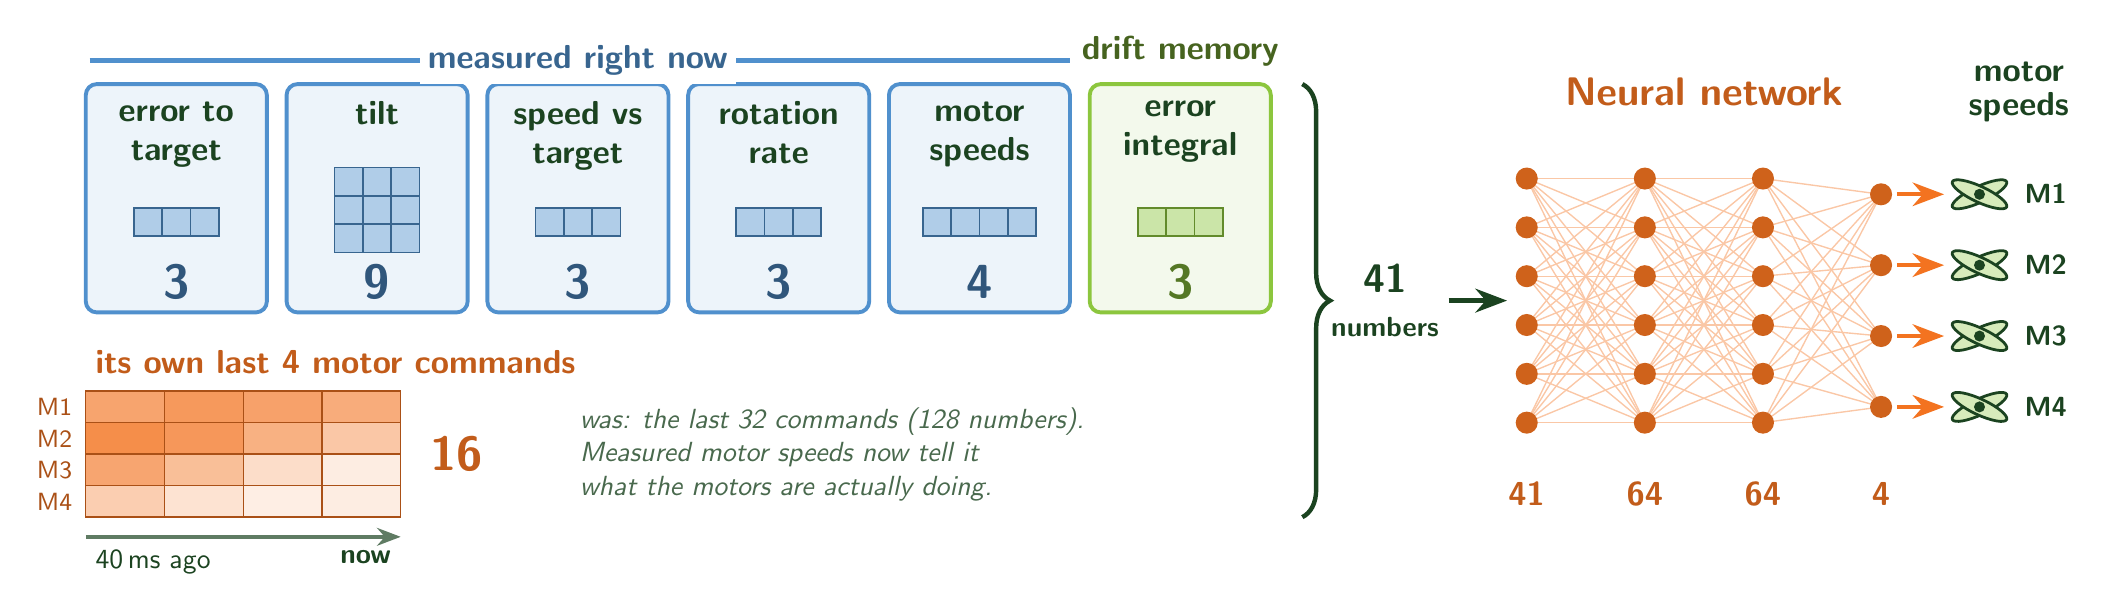
\begin{tikzpicture}
  % ---------- the "right now" groups as cards ----------
  \foreach \x/\ttl/\n/\col in {
      0/{error to\\target}/3/bleu,
      2.55/{tilt}/9/bleu,
      5.1/{speed vs\\target}/3/bleu,
      7.65/{rotation\\rate}/3/bleu,
      10.2/{motor\\speeds}/4/bleu,
      12.75/{error\\integral}/3/vert} {
    \draw[card=\col] (\x-1.15,-1.45) rectangle (\x+1.15,1.45);
    \node[align=center, font=\large\bfseries, text=saclaydk, anchor=north] at (\x,1.35) {\ttl};
    \node[font=\LARGE\bfseries, text=\col!60!black, anchor=south] at (\x,-1.4) {\n};
  }
  % cells inside the cards
  \foreach \x in {0,5.1,7.65} \foreach \i in {-1,0,1}
    \draw[cell=bleu] (\x+\i*\s-\s/2,-0.3-\s/2) rectangle ++(\s,\s);
  \foreach \i in {-1,0,1} \foreach \j in {-1,0,1}
    \draw[cell=bleu] (2.55+\i*\s-\s/2,-0.15+\j*\s-\s/2) rectangle ++(\s,\s);
  \foreach \i in {-1.5,-0.5,0.5,1.5}
    \draw[cell=bleu] (10.2+\i*\s-\s/2,-0.3-\s/2) rectangle ++(\s,\s);
  \foreach \i in {-1,0,1}
    \draw[cell=vert] (12.75+\i*\s-\s/2,-0.3-\s/2) rectangle ++(\s,\s);

  % group headers
  \draw[bleu, line width=1.6pt] (-1.1,1.75) -- (11.35,1.75);
  \node[font=\large\bfseries, text=bleu!70!black, fill=white, inner sep=3pt] at (5.1,1.75) {measured right now};
  \node[font=\large\bfseries, text=vert!50!black, anchor=south] at (12.75,1.55) {drift memory};

  \ifnum\histlen>0
    % ---------- memory: its own last few commands ----------
    \pgfmathtruncatemacro{\nh}{\histlen}
    \pgfmathtruncatemacro{\nnum}{4*\histlen}
    \pgfmathtruncatemacro{\ms}{10*\histlen}
    \def\gw{1.0}
    \node[anchor=south west, font=\large\bfseries, text=mandarine!80!black] at (-1.15,-2.35)
         {its own last \nh\ motor commands};
    \foreach \c in {1,...,\nh} \foreach \r in {0,...,3} {
      \pgfmathtruncatemacro{\v}{max(12, min(85, 45 + 25*sin(\c*23 + \r*70) + 12*sin(\c*61 + \r*20)))}
      \draw[draw=mandarine!70!black, line width=0.5pt, fill=mandarine!\v]
        (-1.15+\c*\gw-\gw, -2.45-\r*0.4) rectangle ++(\gw, -0.4);
    }
    \node[anchor=west, font=\LARGE\bfseries, text=mandarine!80!black] at (-1.15+\nh*\gw+0.25,-3.25) {\nnum};
    \foreach \r/\m in {0/1,1/2,2/3,3/4}
      \node[font=\small, text=mandarine!70!black, anchor=east] at (-1.2,-2.65-\r*0.4) {M\m};
    \draw[-{Stealth[length=3mm]}, line width=1.4pt, saclaydk!70] (-1.15,-4.3) -- (-1.15+\nh*\gw,-4.3);
    \node[anchor=north west, font=\normalsize, text=saclaydk] at (-1.15,-4.35) {\ms\,ms ago};
    \node[anchor=north east, font=\normalsize\bfseries, text=saclaydk] at (-1.15+\nh*\gw,-4.35) {now};
    \node[anchor=west, align=left, font=\normalsize\itshape, text=saclaydk!80] at (5.0,-3.25)
         {was: the last 32 commands (128 numbers).\\Measured motor speeds now tell it\\what the motors are actually doing.};
    \def\ybot{-4.05}
    \def\ny{-1.3}
  \else
    \node[anchor=north west, align=left, font=\normalsize\itshape, text=saclaydk!80] at (-1.15,-1.8)
         {No memory of its own commands (was: the last 32 = 128 numbers).\\
          Measured motor speeds tell it what the motors are actually doing.};
    \def\ybot{-1.45}
    \def\ny{0}
  \fi
  \pgfmathtruncatemacro{\total}{22 + 4*\histlen + 3}

  % ---------- bracket into the network ----------
  \draw[decorate, decoration={brace, amplitude=10pt}, line width=1.6pt, saclaydk]
    (14.3,1.45) -- (14.3,\ybot);
  \node[font=\Large\bfseries, text=saclaydk, align=center] (tot) at (15.35,\ny) {\total\\[-2pt]{\normalsize numbers}};
  \draw[arr, saclaydk] (tot.east) -- (16.9,\ny);

  % ---------- network ----------
  \pgfmathtruncatemacro{\nin}{\histlen > 0 ? 6 : 5}
  \foreach \L/\x/\n/\sp in {0/17.15/\nin/0.62, 1/18.65/6/0.62, 2/20.15/6/0.62, 3/21.65/4/0.9} {
    \foreach \k in {1,...,\n} \coordinate (N\L-\k) at (\x, {\ny + (\n+1)/2*\sp - \k*\sp});
  }
  \foreach \a/\na/\b/\nb in {0/\nin/1/6, 1/6/2/6, 2/6/3/4}
    \foreach \i in {1,...,\na} \foreach \j in {1,...,\nb}
      \draw[mandarine!40, line width=0.5pt] (N\a-\i) -- (N\b-\j);
  \foreach \L/\n in {0/\nin,1/6,2/6,3/4} \foreach \k in {1,...,\n}
    \fill[mandarine!85!black] (N\L-\k) circle (0.14);
  \foreach \x/\lab in {17.15/\total, 18.65/64, 20.15/64, 21.65/4}
    \node[font=\large\bfseries, text=mandarine!80!black] at (\x,\ny-2.45) {\lab};
  \node[font=\Large\bfseries, text=mandarine!80!black] at (19.4,\ny+2.65) {Neural network};

  % ---------- outputs: 4 propellers ----------
  \foreach \k in {1,...,4} {
    \coordinate (P) at ($(N3-\k)+(1.25,0)$);
    \draw[arr, mandarine, line width=1.4pt] ($(N3-\k)+(0.2,0)$) -- ($(P)+(-0.45,0)$);
    \draw[saclaydk, fill=vert!35, line width=1pt, rotate around={25:(P)}] (P) ellipse (0.38 and 0.1);
    \draw[saclaydk, fill=vert!35, line width=1pt, rotate around={-25:(P)}] (P) ellipse (0.38 and 0.1);
    \fill[saclaydk] (P) circle (0.07);
    \node[anchor=west, font=\normalsize\bfseries, text=saclaydk] at ($(P)+(0.45,0)$) {M\k};
  }
  \node[align=center, font=\large\bfseries, text=saclaydk] at (23.4,\ny+2.65) {motor\\[-2pt]speeds};
\end{tikzpicture}
\end{document}
"   (41 inputs)
%   pdflatex -jobname=fig_inputs_none_poster  "\def\histlen{0}% "What the network sees" with measured motor speeds, for the A1 poster.
% One source, two figures (set \histlen before \input):
%   pdflatex -jobname=fig_inputs_short_poster "\def\histlen{4}% "What the network sees" with measured motor speeds, for the A1 poster.
% One source, two figures (set \histlen before \input):
%   pdflatex -jobname=fig_inputs_short_poster "\def\histlen{4}% "What the network sees" with measured motor speeds, for the A1 poster.
% One source, two figures (set \histlen before \input):
%   pdflatex -jobname=fig_inputs_short_poster "\def\histlen{4}\input{fig_inputs_rpm_poster.tex}"   (41 inputs)
%   pdflatex -jobname=fig_inputs_none_poster  "\def\histlen{0}\input{fig_inputs_rpm_poster.tex}"   (25 inputs)
% Compiled on its own it gives the 4-step version. In the poster:
%   \includegraphics[width=\linewidth]{images/fig_inputs_short_poster.pdf}
\documentclass[12pt, border=4pt]{standalone}
\usepackage{tikz}
\usetikzlibrary{arrows.meta,positioning,calc,decorations.pathreplacing}
\renewcommand{\familydefault}{\sfdefault}

\definecolor{saclaydk}{RGB}{27,67,32}
\definecolor{mandarine}{RGB}{243,115,32}
\definecolor{vert}{RGB}{140,198,62}
\definecolor{bleu}{RGB}{80,144,205}
\definecolor{rouge}{RGB}{198,11,70}

\tikzset{
  cell/.style={draw=#1!70!black, fill=#1!45, line width=0.6pt},
  card/.style={draw=#1, fill=#1!10, rounded corners=4pt, line width=1.4pt},
  arr/.style={-{Stealth[length=4mm,width=3mm]}, line width=2pt},
}
\newcommand{\s}{0.36} % cell size
\providecommand{\histlen}{4}

\begin{document}
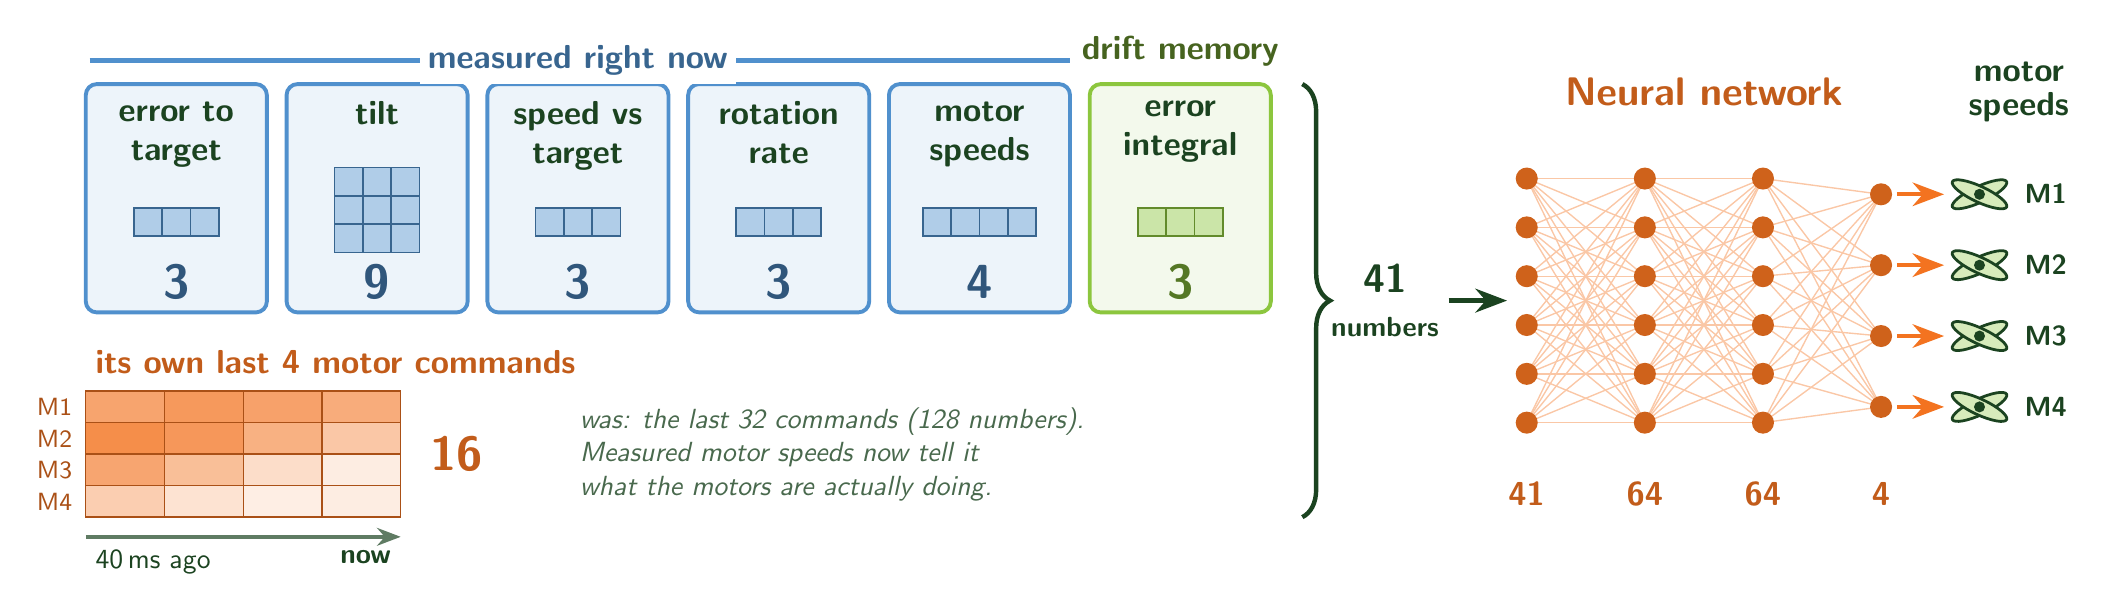
\begin{tikzpicture}
  % ---------- the "right now" groups as cards ----------
  \foreach \x/\ttl/\n/\col in {
      0/{error to\\target}/3/bleu,
      2.55/{tilt}/9/bleu,
      5.1/{speed vs\\target}/3/bleu,
      7.65/{rotation\\rate}/3/bleu,
      10.2/{motor\\speeds}/4/bleu,
      12.75/{error\\integral}/3/vert} {
    \draw[card=\col] (\x-1.15,-1.45) rectangle (\x+1.15,1.45);
    \node[align=center, font=\large\bfseries, text=saclaydk, anchor=north] at (\x,1.35) {\ttl};
    \node[font=\LARGE\bfseries, text=\col!60!black, anchor=south] at (\x,-1.4) {\n};
  }
  % cells inside the cards
  \foreach \x in {0,5.1,7.65} \foreach \i in {-1,0,1}
    \draw[cell=bleu] (\x+\i*\s-\s/2,-0.3-\s/2) rectangle ++(\s,\s);
  \foreach \i in {-1,0,1} \foreach \j in {-1,0,1}
    \draw[cell=bleu] (2.55+\i*\s-\s/2,-0.15+\j*\s-\s/2) rectangle ++(\s,\s);
  \foreach \i in {-1.5,-0.5,0.5,1.5}
    \draw[cell=bleu] (10.2+\i*\s-\s/2,-0.3-\s/2) rectangle ++(\s,\s);
  \foreach \i in {-1,0,1}
    \draw[cell=vert] (12.75+\i*\s-\s/2,-0.3-\s/2) rectangle ++(\s,\s);

  % group headers
  \draw[bleu, line width=1.6pt] (-1.1,1.75) -- (11.35,1.75);
  \node[font=\large\bfseries, text=bleu!70!black, fill=white, inner sep=3pt] at (5.1,1.75) {measured right now};
  \node[font=\large\bfseries, text=vert!50!black, anchor=south] at (12.75,1.55) {drift memory};

  \ifnum\histlen>0
    % ---------- memory: its own last few commands ----------
    \pgfmathtruncatemacro{\nh}{\histlen}
    \pgfmathtruncatemacro{\nnum}{4*\histlen}
    \pgfmathtruncatemacro{\ms}{10*\histlen}
    \def\gw{1.0}
    \node[anchor=south west, font=\large\bfseries, text=mandarine!80!black] at (-1.15,-2.35)
         {its own last \nh\ motor commands};
    \foreach \c in {1,...,\nh} \foreach \r in {0,...,3} {
      \pgfmathtruncatemacro{\v}{max(12, min(85, 45 + 25*sin(\c*23 + \r*70) + 12*sin(\c*61 + \r*20)))}
      \draw[draw=mandarine!70!black, line width=0.5pt, fill=mandarine!\v]
        (-1.15+\c*\gw-\gw, -2.45-\r*0.4) rectangle ++(\gw, -0.4);
    }
    \node[anchor=west, font=\LARGE\bfseries, text=mandarine!80!black] at (-1.15+\nh*\gw+0.25,-3.25) {\nnum};
    \foreach \r/\m in {0/1,1/2,2/3,3/4}
      \node[font=\small, text=mandarine!70!black, anchor=east] at (-1.2,-2.65-\r*0.4) {M\m};
    \draw[-{Stealth[length=3mm]}, line width=1.4pt, saclaydk!70] (-1.15,-4.3) -- (-1.15+\nh*\gw,-4.3);
    \node[anchor=north west, font=\normalsize, text=saclaydk] at (-1.15,-4.35) {\ms\,ms ago};
    \node[anchor=north east, font=\normalsize\bfseries, text=saclaydk] at (-1.15+\nh*\gw,-4.35) {now};
    \node[anchor=west, align=left, font=\normalsize\itshape, text=saclaydk!80] at (5.0,-3.25)
         {was: the last 32 commands (128 numbers).\\Measured motor speeds now tell it\\what the motors are actually doing.};
    \def\ybot{-4.05}
    \def\ny{-1.3}
  \else
    \node[anchor=north west, align=left, font=\normalsize\itshape, text=saclaydk!80] at (-1.15,-1.8)
         {No memory of its own commands (was: the last 32 = 128 numbers).\\
          Measured motor speeds tell it what the motors are actually doing.};
    \def\ybot{-1.45}
    \def\ny{0}
  \fi
  \pgfmathtruncatemacro{\total}{22 + 4*\histlen + 3}

  % ---------- bracket into the network ----------
  \draw[decorate, decoration={brace, amplitude=10pt}, line width=1.6pt, saclaydk]
    (14.3,1.45) -- (14.3,\ybot);
  \node[font=\Large\bfseries, text=saclaydk, align=center] (tot) at (15.35,\ny) {\total\\[-2pt]{\normalsize numbers}};
  \draw[arr, saclaydk] (tot.east) -- (16.9,\ny);

  % ---------- network ----------
  \pgfmathtruncatemacro{\nin}{\histlen > 0 ? 6 : 5}
  \foreach \L/\x/\n/\sp in {0/17.15/\nin/0.62, 1/18.65/6/0.62, 2/20.15/6/0.62, 3/21.65/4/0.9} {
    \foreach \k in {1,...,\n} \coordinate (N\L-\k) at (\x, {\ny + (\n+1)/2*\sp - \k*\sp});
  }
  \foreach \a/\na/\b/\nb in {0/\nin/1/6, 1/6/2/6, 2/6/3/4}
    \foreach \i in {1,...,\na} \foreach \j in {1,...,\nb}
      \draw[mandarine!40, line width=0.5pt] (N\a-\i) -- (N\b-\j);
  \foreach \L/\n in {0/\nin,1/6,2/6,3/4} \foreach \k in {1,...,\n}
    \fill[mandarine!85!black] (N\L-\k) circle (0.14);
  \foreach \x/\lab in {17.15/\total, 18.65/64, 20.15/64, 21.65/4}
    \node[font=\large\bfseries, text=mandarine!80!black] at (\x,\ny-2.45) {\lab};
  \node[font=\Large\bfseries, text=mandarine!80!black] at (19.4,\ny+2.65) {Neural network};

  % ---------- outputs: 4 propellers ----------
  \foreach \k in {1,...,4} {
    \coordinate (P) at ($(N3-\k)+(1.25,0)$);
    \draw[arr, mandarine, line width=1.4pt] ($(N3-\k)+(0.2,0)$) -- ($(P)+(-0.45,0)$);
    \draw[saclaydk, fill=vert!35, line width=1pt, rotate around={25:(P)}] (P) ellipse (0.38 and 0.1);
    \draw[saclaydk, fill=vert!35, line width=1pt, rotate around={-25:(P)}] (P) ellipse (0.38 and 0.1);
    \fill[saclaydk] (P) circle (0.07);
    \node[anchor=west, font=\normalsize\bfseries, text=saclaydk] at ($(P)+(0.45,0)$) {M\k};
  }
  \node[align=center, font=\large\bfseries, text=saclaydk] at (23.4,\ny+2.65) {motor\\[-2pt]speeds};
\end{tikzpicture}
\end{document}
"   (41 inputs)
%   pdflatex -jobname=fig_inputs_none_poster  "\def\histlen{0}% "What the network sees" with measured motor speeds, for the A1 poster.
% One source, two figures (set \histlen before \input):
%   pdflatex -jobname=fig_inputs_short_poster "\def\histlen{4}\input{fig_inputs_rpm_poster.tex}"   (41 inputs)
%   pdflatex -jobname=fig_inputs_none_poster  "\def\histlen{0}\input{fig_inputs_rpm_poster.tex}"   (25 inputs)
% Compiled on its own it gives the 4-step version. In the poster:
%   \includegraphics[width=\linewidth]{images/fig_inputs_short_poster.pdf}
\documentclass[12pt, border=4pt]{standalone}
\usepackage{tikz}
\usetikzlibrary{arrows.meta,positioning,calc,decorations.pathreplacing}
\renewcommand{\familydefault}{\sfdefault}

\definecolor{saclaydk}{RGB}{27,67,32}
\definecolor{mandarine}{RGB}{243,115,32}
\definecolor{vert}{RGB}{140,198,62}
\definecolor{bleu}{RGB}{80,144,205}
\definecolor{rouge}{RGB}{198,11,70}

\tikzset{
  cell/.style={draw=#1!70!black, fill=#1!45, line width=0.6pt},
  card/.style={draw=#1, fill=#1!10, rounded corners=4pt, line width=1.4pt},
  arr/.style={-{Stealth[length=4mm,width=3mm]}, line width=2pt},
}
\newcommand{\s}{0.36} % cell size
\providecommand{\histlen}{4}

\begin{document}
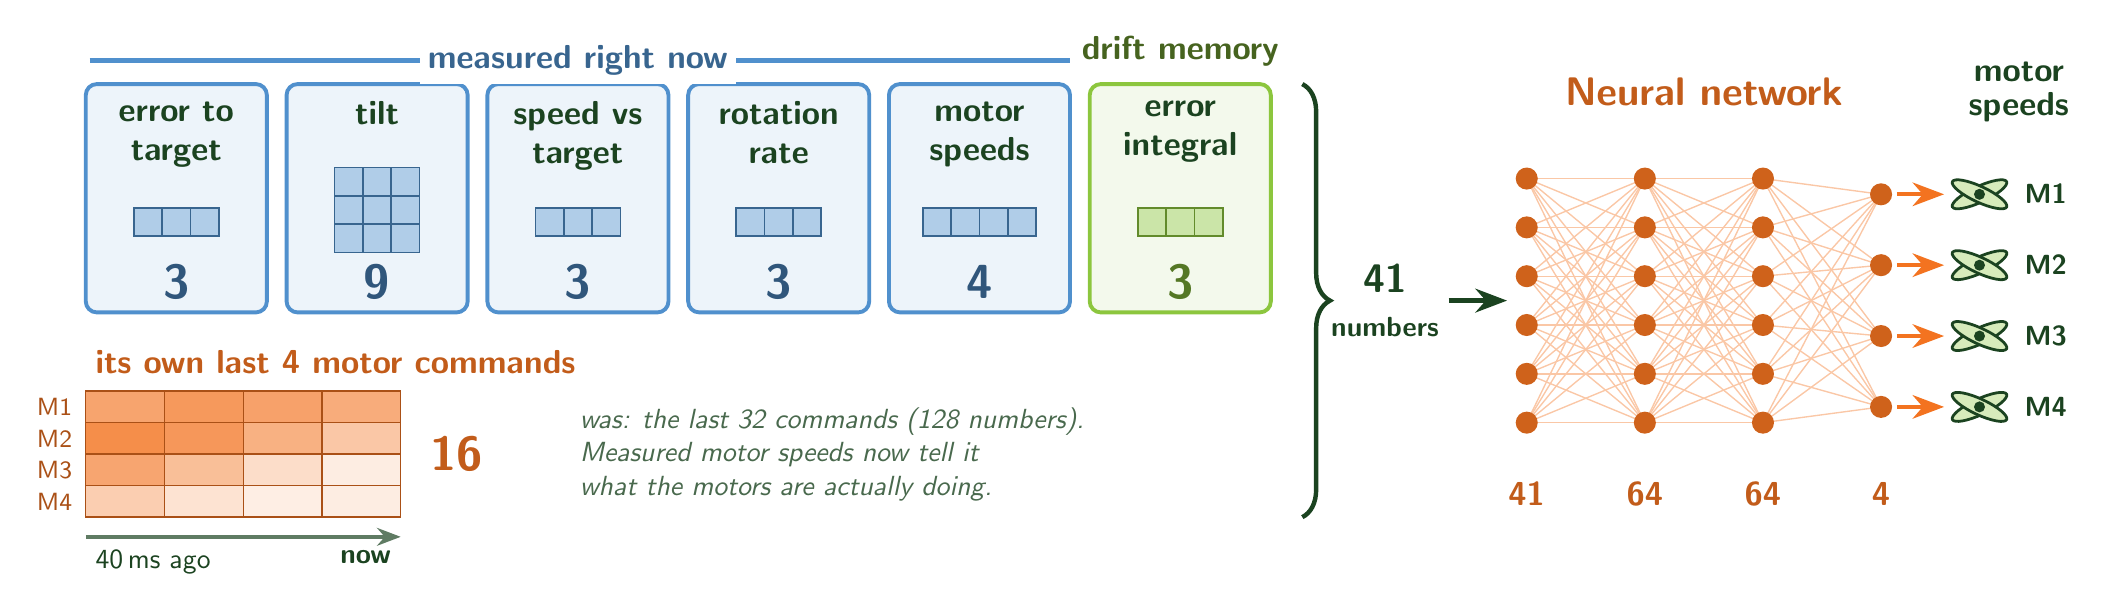
\begin{tikzpicture}
  % ---------- the "right now" groups as cards ----------
  \foreach \x/\ttl/\n/\col in {
      0/{error to\\target}/3/bleu,
      2.55/{tilt}/9/bleu,
      5.1/{speed vs\\target}/3/bleu,
      7.65/{rotation\\rate}/3/bleu,
      10.2/{motor\\speeds}/4/bleu,
      12.75/{error\\integral}/3/vert} {
    \draw[card=\col] (\x-1.15,-1.45) rectangle (\x+1.15,1.45);
    \node[align=center, font=\large\bfseries, text=saclaydk, anchor=north] at (\x,1.35) {\ttl};
    \node[font=\LARGE\bfseries, text=\col!60!black, anchor=south] at (\x,-1.4) {\n};
  }
  % cells inside the cards
  \foreach \x in {0,5.1,7.65} \foreach \i in {-1,0,1}
    \draw[cell=bleu] (\x+\i*\s-\s/2,-0.3-\s/2) rectangle ++(\s,\s);
  \foreach \i in {-1,0,1} \foreach \j in {-1,0,1}
    \draw[cell=bleu] (2.55+\i*\s-\s/2,-0.15+\j*\s-\s/2) rectangle ++(\s,\s);
  \foreach \i in {-1.5,-0.5,0.5,1.5}
    \draw[cell=bleu] (10.2+\i*\s-\s/2,-0.3-\s/2) rectangle ++(\s,\s);
  \foreach \i in {-1,0,1}
    \draw[cell=vert] (12.75+\i*\s-\s/2,-0.3-\s/2) rectangle ++(\s,\s);

  % group headers
  \draw[bleu, line width=1.6pt] (-1.1,1.75) -- (11.35,1.75);
  \node[font=\large\bfseries, text=bleu!70!black, fill=white, inner sep=3pt] at (5.1,1.75) {measured right now};
  \node[font=\large\bfseries, text=vert!50!black, anchor=south] at (12.75,1.55) {drift memory};

  \ifnum\histlen>0
    % ---------- memory: its own last few commands ----------
    \pgfmathtruncatemacro{\nh}{\histlen}
    \pgfmathtruncatemacro{\nnum}{4*\histlen}
    \pgfmathtruncatemacro{\ms}{10*\histlen}
    \def\gw{1.0}
    \node[anchor=south west, font=\large\bfseries, text=mandarine!80!black] at (-1.15,-2.35)
         {its own last \nh\ motor commands};
    \foreach \c in {1,...,\nh} \foreach \r in {0,...,3} {
      \pgfmathtruncatemacro{\v}{max(12, min(85, 45 + 25*sin(\c*23 + \r*70) + 12*sin(\c*61 + \r*20)))}
      \draw[draw=mandarine!70!black, line width=0.5pt, fill=mandarine!\v]
        (-1.15+\c*\gw-\gw, -2.45-\r*0.4) rectangle ++(\gw, -0.4);
    }
    \node[anchor=west, font=\LARGE\bfseries, text=mandarine!80!black] at (-1.15+\nh*\gw+0.25,-3.25) {\nnum};
    \foreach \r/\m in {0/1,1/2,2/3,3/4}
      \node[font=\small, text=mandarine!70!black, anchor=east] at (-1.2,-2.65-\r*0.4) {M\m};
    \draw[-{Stealth[length=3mm]}, line width=1.4pt, saclaydk!70] (-1.15,-4.3) -- (-1.15+\nh*\gw,-4.3);
    \node[anchor=north west, font=\normalsize, text=saclaydk] at (-1.15,-4.35) {\ms\,ms ago};
    \node[anchor=north east, font=\normalsize\bfseries, text=saclaydk] at (-1.15+\nh*\gw,-4.35) {now};
    \node[anchor=west, align=left, font=\normalsize\itshape, text=saclaydk!80] at (5.0,-3.25)
         {was: the last 32 commands (128 numbers).\\Measured motor speeds now tell it\\what the motors are actually doing.};
    \def\ybot{-4.05}
    \def\ny{-1.3}
  \else
    \node[anchor=north west, align=left, font=\normalsize\itshape, text=saclaydk!80] at (-1.15,-1.8)
         {No memory of its own commands (was: the last 32 = 128 numbers).\\
          Measured motor speeds tell it what the motors are actually doing.};
    \def\ybot{-1.45}
    \def\ny{0}
  \fi
  \pgfmathtruncatemacro{\total}{22 + 4*\histlen + 3}

  % ---------- bracket into the network ----------
  \draw[decorate, decoration={brace, amplitude=10pt}, line width=1.6pt, saclaydk]
    (14.3,1.45) -- (14.3,\ybot);
  \node[font=\Large\bfseries, text=saclaydk, align=center] (tot) at (15.35,\ny) {\total\\[-2pt]{\normalsize numbers}};
  \draw[arr, saclaydk] (tot.east) -- (16.9,\ny);

  % ---------- network ----------
  \pgfmathtruncatemacro{\nin}{\histlen > 0 ? 6 : 5}
  \foreach \L/\x/\n/\sp in {0/17.15/\nin/0.62, 1/18.65/6/0.62, 2/20.15/6/0.62, 3/21.65/4/0.9} {
    \foreach \k in {1,...,\n} \coordinate (N\L-\k) at (\x, {\ny + (\n+1)/2*\sp - \k*\sp});
  }
  \foreach \a/\na/\b/\nb in {0/\nin/1/6, 1/6/2/6, 2/6/3/4}
    \foreach \i in {1,...,\na} \foreach \j in {1,...,\nb}
      \draw[mandarine!40, line width=0.5pt] (N\a-\i) -- (N\b-\j);
  \foreach \L/\n in {0/\nin,1/6,2/6,3/4} \foreach \k in {1,...,\n}
    \fill[mandarine!85!black] (N\L-\k) circle (0.14);
  \foreach \x/\lab in {17.15/\total, 18.65/64, 20.15/64, 21.65/4}
    \node[font=\large\bfseries, text=mandarine!80!black] at (\x,\ny-2.45) {\lab};
  \node[font=\Large\bfseries, text=mandarine!80!black] at (19.4,\ny+2.65) {Neural network};

  % ---------- outputs: 4 propellers ----------
  \foreach \k in {1,...,4} {
    \coordinate (P) at ($(N3-\k)+(1.25,0)$);
    \draw[arr, mandarine, line width=1.4pt] ($(N3-\k)+(0.2,0)$) -- ($(P)+(-0.45,0)$);
    \draw[saclaydk, fill=vert!35, line width=1pt, rotate around={25:(P)}] (P) ellipse (0.38 and 0.1);
    \draw[saclaydk, fill=vert!35, line width=1pt, rotate around={-25:(P)}] (P) ellipse (0.38 and 0.1);
    \fill[saclaydk] (P) circle (0.07);
    \node[anchor=west, font=\normalsize\bfseries, text=saclaydk] at ($(P)+(0.45,0)$) {M\k};
  }
  \node[align=center, font=\large\bfseries, text=saclaydk] at (23.4,\ny+2.65) {motor\\[-2pt]speeds};
\end{tikzpicture}
\end{document}
"   (25 inputs)
% Compiled on its own it gives the 4-step version. In the poster:
%   \includegraphics[width=\linewidth]{images/fig_inputs_short_poster.pdf}
\documentclass[12pt, border=4pt]{standalone}
\usepackage{tikz}
\usetikzlibrary{arrows.meta,positioning,calc,decorations.pathreplacing}
\renewcommand{\familydefault}{\sfdefault}

\definecolor{saclaydk}{RGB}{27,67,32}
\definecolor{mandarine}{RGB}{243,115,32}
\definecolor{vert}{RGB}{140,198,62}
\definecolor{bleu}{RGB}{80,144,205}
\definecolor{rouge}{RGB}{198,11,70}

\tikzset{
  cell/.style={draw=#1!70!black, fill=#1!45, line width=0.6pt},
  card/.style={draw=#1, fill=#1!10, rounded corners=4pt, line width=1.4pt},
  arr/.style={-{Stealth[length=4mm,width=3mm]}, line width=2pt},
}
\newcommand{\s}{0.36} % cell size
\providecommand{\histlen}{4}

\begin{document}
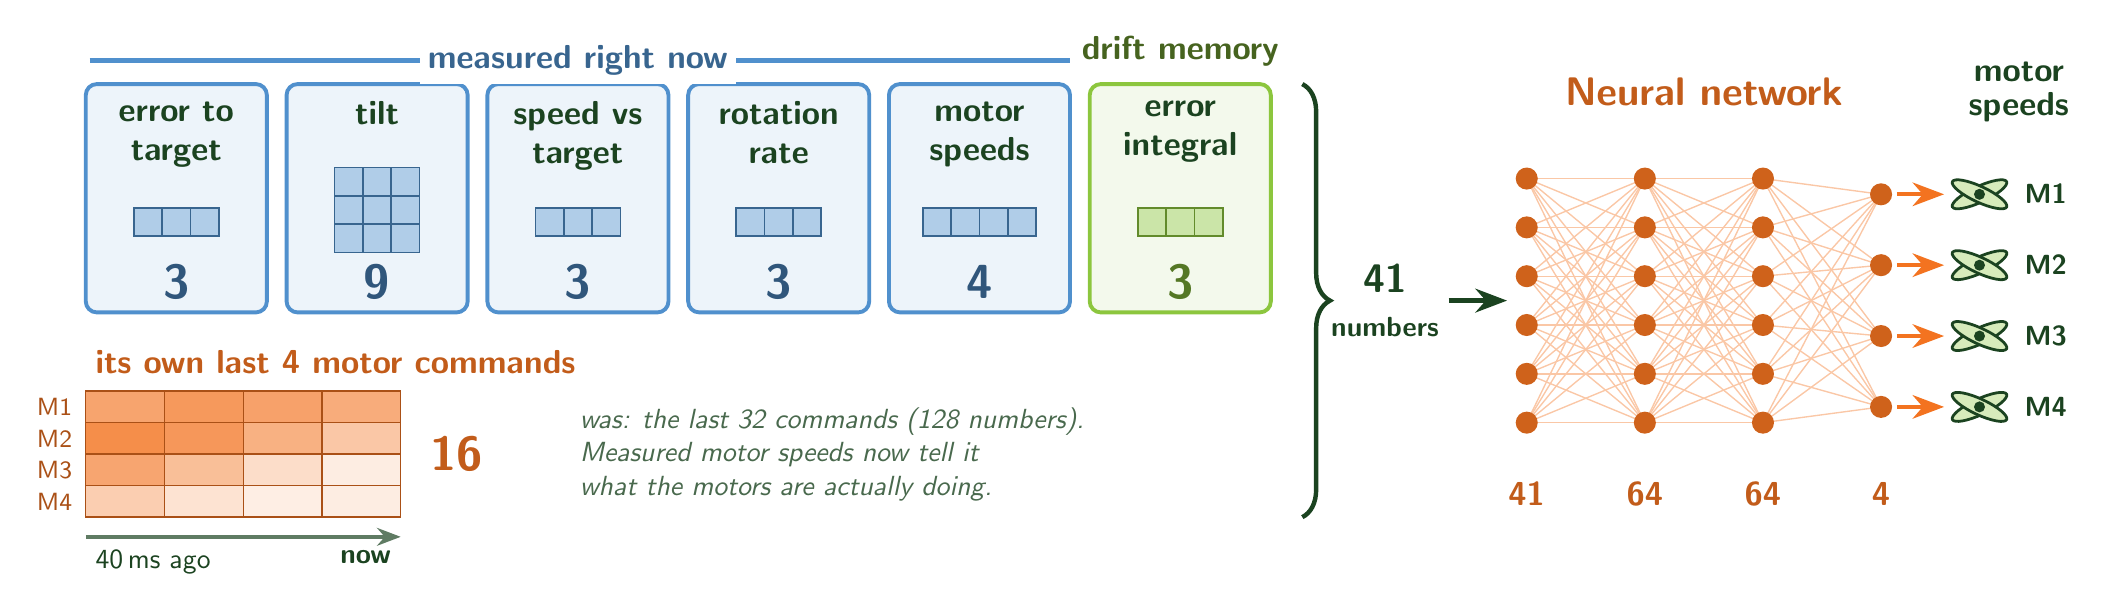
\begin{tikzpicture}
  % ---------- the "right now" groups as cards ----------
  \foreach \x/\ttl/\n/\col in {
      0/{error to\\target}/3/bleu,
      2.55/{tilt}/9/bleu,
      5.1/{speed vs\\target}/3/bleu,
      7.65/{rotation\\rate}/3/bleu,
      10.2/{motor\\speeds}/4/bleu,
      12.75/{error\\integral}/3/vert} {
    \draw[card=\col] (\x-1.15,-1.45) rectangle (\x+1.15,1.45);
    \node[align=center, font=\large\bfseries, text=saclaydk, anchor=north] at (\x,1.35) {\ttl};
    \node[font=\LARGE\bfseries, text=\col!60!black, anchor=south] at (\x,-1.4) {\n};
  }
  % cells inside the cards
  \foreach \x in {0,5.1,7.65} \foreach \i in {-1,0,1}
    \draw[cell=bleu] (\x+\i*\s-\s/2,-0.3-\s/2) rectangle ++(\s,\s);
  \foreach \i in {-1,0,1} \foreach \j in {-1,0,1}
    \draw[cell=bleu] (2.55+\i*\s-\s/2,-0.15+\j*\s-\s/2) rectangle ++(\s,\s);
  \foreach \i in {-1.5,-0.5,0.5,1.5}
    \draw[cell=bleu] (10.2+\i*\s-\s/2,-0.3-\s/2) rectangle ++(\s,\s);
  \foreach \i in {-1,0,1}
    \draw[cell=vert] (12.75+\i*\s-\s/2,-0.3-\s/2) rectangle ++(\s,\s);

  % group headers
  \draw[bleu, line width=1.6pt] (-1.1,1.75) -- (11.35,1.75);
  \node[font=\large\bfseries, text=bleu!70!black, fill=white, inner sep=3pt] at (5.1,1.75) {measured right now};
  \node[font=\large\bfseries, text=vert!50!black, anchor=south] at (12.75,1.55) {drift memory};

  \ifnum\histlen>0
    % ---------- memory: its own last few commands ----------
    \pgfmathtruncatemacro{\nh}{\histlen}
    \pgfmathtruncatemacro{\nnum}{4*\histlen}
    \pgfmathtruncatemacro{\ms}{10*\histlen}
    \def\gw{1.0}
    \node[anchor=south west, font=\large\bfseries, text=mandarine!80!black] at (-1.15,-2.35)
         {its own last \nh\ motor commands};
    \foreach \c in {1,...,\nh} \foreach \r in {0,...,3} {
      \pgfmathtruncatemacro{\v}{max(12, min(85, 45 + 25*sin(\c*23 + \r*70) + 12*sin(\c*61 + \r*20)))}
      \draw[draw=mandarine!70!black, line width=0.5pt, fill=mandarine!\v]
        (-1.15+\c*\gw-\gw, -2.45-\r*0.4) rectangle ++(\gw, -0.4);
    }
    \node[anchor=west, font=\LARGE\bfseries, text=mandarine!80!black] at (-1.15+\nh*\gw+0.25,-3.25) {\nnum};
    \foreach \r/\m in {0/1,1/2,2/3,3/4}
      \node[font=\small, text=mandarine!70!black, anchor=east] at (-1.2,-2.65-\r*0.4) {M\m};
    \draw[-{Stealth[length=3mm]}, line width=1.4pt, saclaydk!70] (-1.15,-4.3) -- (-1.15+\nh*\gw,-4.3);
    \node[anchor=north west, font=\normalsize, text=saclaydk] at (-1.15,-4.35) {\ms\,ms ago};
    \node[anchor=north east, font=\normalsize\bfseries, text=saclaydk] at (-1.15+\nh*\gw,-4.35) {now};
    \node[anchor=west, align=left, font=\normalsize\itshape, text=saclaydk!80] at (5.0,-3.25)
         {was: the last 32 commands (128 numbers).\\Measured motor speeds now tell it\\what the motors are actually doing.};
    \def\ybot{-4.05}
    \def\ny{-1.3}
  \else
    \node[anchor=north west, align=left, font=\normalsize\itshape, text=saclaydk!80] at (-1.15,-1.8)
         {No memory of its own commands (was: the last 32 = 128 numbers).\\
          Measured motor speeds tell it what the motors are actually doing.};
    \def\ybot{-1.45}
    \def\ny{0}
  \fi
  \pgfmathtruncatemacro{\total}{22 + 4*\histlen + 3}

  % ---------- bracket into the network ----------
  \draw[decorate, decoration={brace, amplitude=10pt}, line width=1.6pt, saclaydk]
    (14.3,1.45) -- (14.3,\ybot);
  \node[font=\Large\bfseries, text=saclaydk, align=center] (tot) at (15.35,\ny) {\total\\[-2pt]{\normalsize numbers}};
  \draw[arr, saclaydk] (tot.east) -- (16.9,\ny);

  % ---------- network ----------
  \pgfmathtruncatemacro{\nin}{\histlen > 0 ? 6 : 5}
  \foreach \L/\x/\n/\sp in {0/17.15/\nin/0.62, 1/18.65/6/0.62, 2/20.15/6/0.62, 3/21.65/4/0.9} {
    \foreach \k in {1,...,\n} \coordinate (N\L-\k) at (\x, {\ny + (\n+1)/2*\sp - \k*\sp});
  }
  \foreach \a/\na/\b/\nb in {0/\nin/1/6, 1/6/2/6, 2/6/3/4}
    \foreach \i in {1,...,\na} \foreach \j in {1,...,\nb}
      \draw[mandarine!40, line width=0.5pt] (N\a-\i) -- (N\b-\j);
  \foreach \L/\n in {0/\nin,1/6,2/6,3/4} \foreach \k in {1,...,\n}
    \fill[mandarine!85!black] (N\L-\k) circle (0.14);
  \foreach \x/\lab in {17.15/\total, 18.65/64, 20.15/64, 21.65/4}
    \node[font=\large\bfseries, text=mandarine!80!black] at (\x,\ny-2.45) {\lab};
  \node[font=\Large\bfseries, text=mandarine!80!black] at (19.4,\ny+2.65) {Neural network};

  % ---------- outputs: 4 propellers ----------
  \foreach \k in {1,...,4} {
    \coordinate (P) at ($(N3-\k)+(1.25,0)$);
    \draw[arr, mandarine, line width=1.4pt] ($(N3-\k)+(0.2,0)$) -- ($(P)+(-0.45,0)$);
    \draw[saclaydk, fill=vert!35, line width=1pt, rotate around={25:(P)}] (P) ellipse (0.38 and 0.1);
    \draw[saclaydk, fill=vert!35, line width=1pt, rotate around={-25:(P)}] (P) ellipse (0.38 and 0.1);
    \fill[saclaydk] (P) circle (0.07);
    \node[anchor=west, font=\normalsize\bfseries, text=saclaydk] at ($(P)+(0.45,0)$) {M\k};
  }
  \node[align=center, font=\large\bfseries, text=saclaydk] at (23.4,\ny+2.65) {motor\\[-2pt]speeds};
\end{tikzpicture}
\end{document}
"   (41 inputs)
%   pdflatex -jobname=fig_inputs_none_poster  "\def\histlen{0}% "What the network sees" with measured motor speeds, for the A1 poster.
% One source, two figures (set \histlen before \input):
%   pdflatex -jobname=fig_inputs_short_poster "\def\histlen{4}% "What the network sees" with measured motor speeds, for the A1 poster.
% One source, two figures (set \histlen before \input):
%   pdflatex -jobname=fig_inputs_short_poster "\def\histlen{4}\input{fig_inputs_rpm_poster.tex}"   (41 inputs)
%   pdflatex -jobname=fig_inputs_none_poster  "\def\histlen{0}\input{fig_inputs_rpm_poster.tex}"   (25 inputs)
% Compiled on its own it gives the 4-step version. In the poster:
%   \includegraphics[width=\linewidth]{images/fig_inputs_short_poster.pdf}
\documentclass[12pt, border=4pt]{standalone}
\usepackage{tikz}
\usetikzlibrary{arrows.meta,positioning,calc,decorations.pathreplacing}
\renewcommand{\familydefault}{\sfdefault}

\definecolor{saclaydk}{RGB}{27,67,32}
\definecolor{mandarine}{RGB}{243,115,32}
\definecolor{vert}{RGB}{140,198,62}
\definecolor{bleu}{RGB}{80,144,205}
\definecolor{rouge}{RGB}{198,11,70}

\tikzset{
  cell/.style={draw=#1!70!black, fill=#1!45, line width=0.6pt},
  card/.style={draw=#1, fill=#1!10, rounded corners=4pt, line width=1.4pt},
  arr/.style={-{Stealth[length=4mm,width=3mm]}, line width=2pt},
}
\newcommand{\s}{0.36} % cell size
\providecommand{\histlen}{4}

\begin{document}
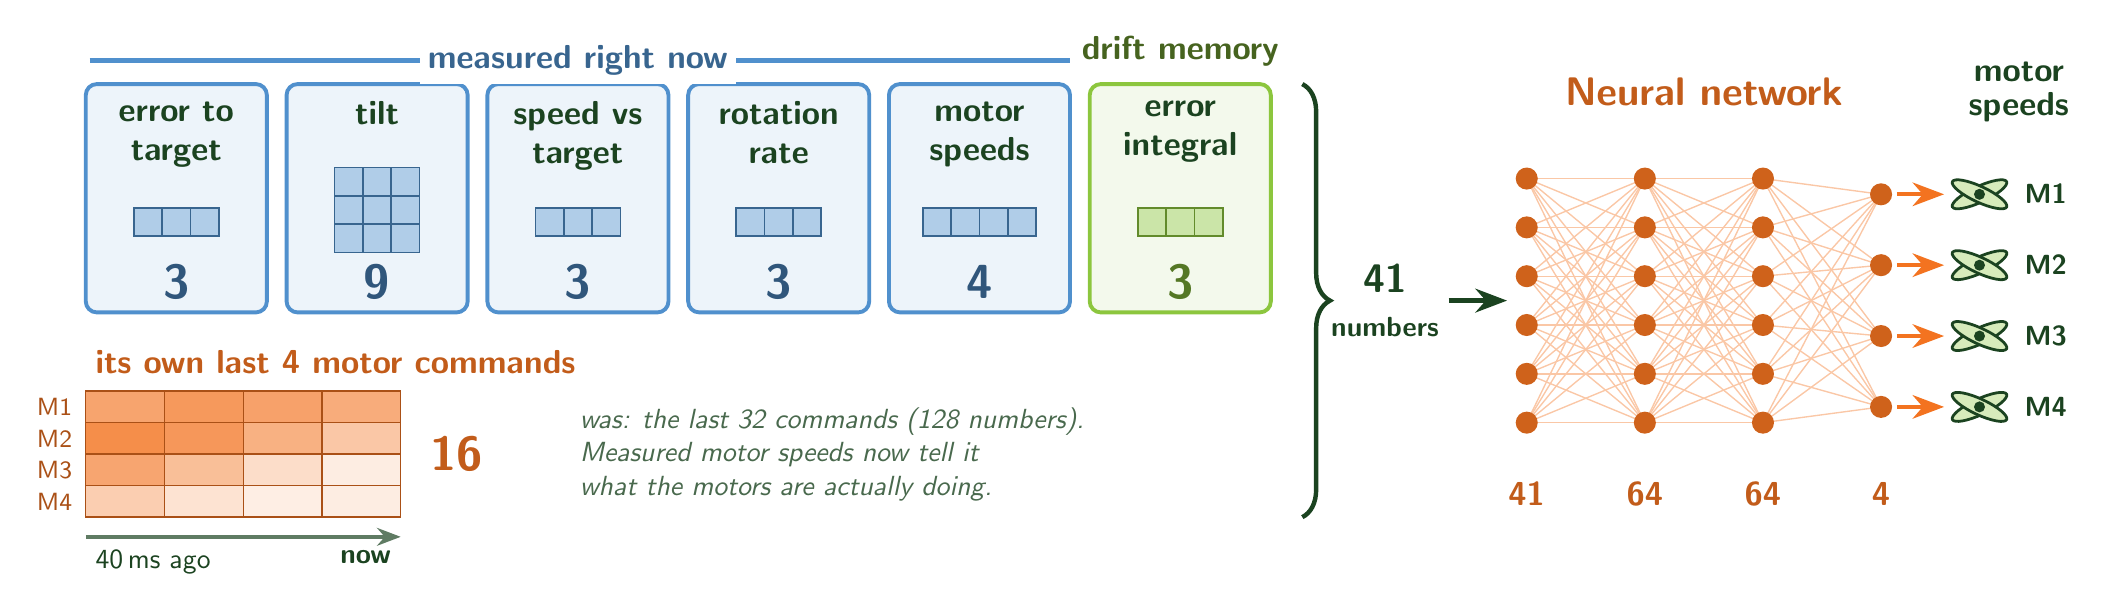
\begin{tikzpicture}
  % ---------- the "right now" groups as cards ----------
  \foreach \x/\ttl/\n/\col in {
      0/{error to\\target}/3/bleu,
      2.55/{tilt}/9/bleu,
      5.1/{speed vs\\target}/3/bleu,
      7.65/{rotation\\rate}/3/bleu,
      10.2/{motor\\speeds}/4/bleu,
      12.75/{error\\integral}/3/vert} {
    \draw[card=\col] (\x-1.15,-1.45) rectangle (\x+1.15,1.45);
    \node[align=center, font=\large\bfseries, text=saclaydk, anchor=north] at (\x,1.35) {\ttl};
    \node[font=\LARGE\bfseries, text=\col!60!black, anchor=south] at (\x,-1.4) {\n};
  }
  % cells inside the cards
  \foreach \x in {0,5.1,7.65} \foreach \i in {-1,0,1}
    \draw[cell=bleu] (\x+\i*\s-\s/2,-0.3-\s/2) rectangle ++(\s,\s);
  \foreach \i in {-1,0,1} \foreach \j in {-1,0,1}
    \draw[cell=bleu] (2.55+\i*\s-\s/2,-0.15+\j*\s-\s/2) rectangle ++(\s,\s);
  \foreach \i in {-1.5,-0.5,0.5,1.5}
    \draw[cell=bleu] (10.2+\i*\s-\s/2,-0.3-\s/2) rectangle ++(\s,\s);
  \foreach \i in {-1,0,1}
    \draw[cell=vert] (12.75+\i*\s-\s/2,-0.3-\s/2) rectangle ++(\s,\s);

  % group headers
  \draw[bleu, line width=1.6pt] (-1.1,1.75) -- (11.35,1.75);
  \node[font=\large\bfseries, text=bleu!70!black, fill=white, inner sep=3pt] at (5.1,1.75) {measured right now};
  \node[font=\large\bfseries, text=vert!50!black, anchor=south] at (12.75,1.55) {drift memory};

  \ifnum\histlen>0
    % ---------- memory: its own last few commands ----------
    \pgfmathtruncatemacro{\nh}{\histlen}
    \pgfmathtruncatemacro{\nnum}{4*\histlen}
    \pgfmathtruncatemacro{\ms}{10*\histlen}
    \def\gw{1.0}
    \node[anchor=south west, font=\large\bfseries, text=mandarine!80!black] at (-1.15,-2.35)
         {its own last \nh\ motor commands};
    \foreach \c in {1,...,\nh} \foreach \r in {0,...,3} {
      \pgfmathtruncatemacro{\v}{max(12, min(85, 45 + 25*sin(\c*23 + \r*70) + 12*sin(\c*61 + \r*20)))}
      \draw[draw=mandarine!70!black, line width=0.5pt, fill=mandarine!\v]
        (-1.15+\c*\gw-\gw, -2.45-\r*0.4) rectangle ++(\gw, -0.4);
    }
    \node[anchor=west, font=\LARGE\bfseries, text=mandarine!80!black] at (-1.15+\nh*\gw+0.25,-3.25) {\nnum};
    \foreach \r/\m in {0/1,1/2,2/3,3/4}
      \node[font=\small, text=mandarine!70!black, anchor=east] at (-1.2,-2.65-\r*0.4) {M\m};
    \draw[-{Stealth[length=3mm]}, line width=1.4pt, saclaydk!70] (-1.15,-4.3) -- (-1.15+\nh*\gw,-4.3);
    \node[anchor=north west, font=\normalsize, text=saclaydk] at (-1.15,-4.35) {\ms\,ms ago};
    \node[anchor=north east, font=\normalsize\bfseries, text=saclaydk] at (-1.15+\nh*\gw,-4.35) {now};
    \node[anchor=west, align=left, font=\normalsize\itshape, text=saclaydk!80] at (5.0,-3.25)
         {was: the last 32 commands (128 numbers).\\Measured motor speeds now tell it\\what the motors are actually doing.};
    \def\ybot{-4.05}
    \def\ny{-1.3}
  \else
    \node[anchor=north west, align=left, font=\normalsize\itshape, text=saclaydk!80] at (-1.15,-1.8)
         {No memory of its own commands (was: the last 32 = 128 numbers).\\
          Measured motor speeds tell it what the motors are actually doing.};
    \def\ybot{-1.45}
    \def\ny{0}
  \fi
  \pgfmathtruncatemacro{\total}{22 + 4*\histlen + 3}

  % ---------- bracket into the network ----------
  \draw[decorate, decoration={brace, amplitude=10pt}, line width=1.6pt, saclaydk]
    (14.3,1.45) -- (14.3,\ybot);
  \node[font=\Large\bfseries, text=saclaydk, align=center] (tot) at (15.35,\ny) {\total\\[-2pt]{\normalsize numbers}};
  \draw[arr, saclaydk] (tot.east) -- (16.9,\ny);

  % ---------- network ----------
  \pgfmathtruncatemacro{\nin}{\histlen > 0 ? 6 : 5}
  \foreach \L/\x/\n/\sp in {0/17.15/\nin/0.62, 1/18.65/6/0.62, 2/20.15/6/0.62, 3/21.65/4/0.9} {
    \foreach \k in {1,...,\n} \coordinate (N\L-\k) at (\x, {\ny + (\n+1)/2*\sp - \k*\sp});
  }
  \foreach \a/\na/\b/\nb in {0/\nin/1/6, 1/6/2/6, 2/6/3/4}
    \foreach \i in {1,...,\na} \foreach \j in {1,...,\nb}
      \draw[mandarine!40, line width=0.5pt] (N\a-\i) -- (N\b-\j);
  \foreach \L/\n in {0/\nin,1/6,2/6,3/4} \foreach \k in {1,...,\n}
    \fill[mandarine!85!black] (N\L-\k) circle (0.14);
  \foreach \x/\lab in {17.15/\total, 18.65/64, 20.15/64, 21.65/4}
    \node[font=\large\bfseries, text=mandarine!80!black] at (\x,\ny-2.45) {\lab};
  \node[font=\Large\bfseries, text=mandarine!80!black] at (19.4,\ny+2.65) {Neural network};

  % ---------- outputs: 4 propellers ----------
  \foreach \k in {1,...,4} {
    \coordinate (P) at ($(N3-\k)+(1.25,0)$);
    \draw[arr, mandarine, line width=1.4pt] ($(N3-\k)+(0.2,0)$) -- ($(P)+(-0.45,0)$);
    \draw[saclaydk, fill=vert!35, line width=1pt, rotate around={25:(P)}] (P) ellipse (0.38 and 0.1);
    \draw[saclaydk, fill=vert!35, line width=1pt, rotate around={-25:(P)}] (P) ellipse (0.38 and 0.1);
    \fill[saclaydk] (P) circle (0.07);
    \node[anchor=west, font=\normalsize\bfseries, text=saclaydk] at ($(P)+(0.45,0)$) {M\k};
  }
  \node[align=center, font=\large\bfseries, text=saclaydk] at (23.4,\ny+2.65) {motor\\[-2pt]speeds};
\end{tikzpicture}
\end{document}
"   (41 inputs)
%   pdflatex -jobname=fig_inputs_none_poster  "\def\histlen{0}% "What the network sees" with measured motor speeds, for the A1 poster.
% One source, two figures (set \histlen before \input):
%   pdflatex -jobname=fig_inputs_short_poster "\def\histlen{4}\input{fig_inputs_rpm_poster.tex}"   (41 inputs)
%   pdflatex -jobname=fig_inputs_none_poster  "\def\histlen{0}\input{fig_inputs_rpm_poster.tex}"   (25 inputs)
% Compiled on its own it gives the 4-step version. In the poster:
%   \includegraphics[width=\linewidth]{images/fig_inputs_short_poster.pdf}
\documentclass[12pt, border=4pt]{standalone}
\usepackage{tikz}
\usetikzlibrary{arrows.meta,positioning,calc,decorations.pathreplacing}
\renewcommand{\familydefault}{\sfdefault}

\definecolor{saclaydk}{RGB}{27,67,32}
\definecolor{mandarine}{RGB}{243,115,32}
\definecolor{vert}{RGB}{140,198,62}
\definecolor{bleu}{RGB}{80,144,205}
\definecolor{rouge}{RGB}{198,11,70}

\tikzset{
  cell/.style={draw=#1!70!black, fill=#1!45, line width=0.6pt},
  card/.style={draw=#1, fill=#1!10, rounded corners=4pt, line width=1.4pt},
  arr/.style={-{Stealth[length=4mm,width=3mm]}, line width=2pt},
}
\newcommand{\s}{0.36} % cell size
\providecommand{\histlen}{4}

\begin{document}
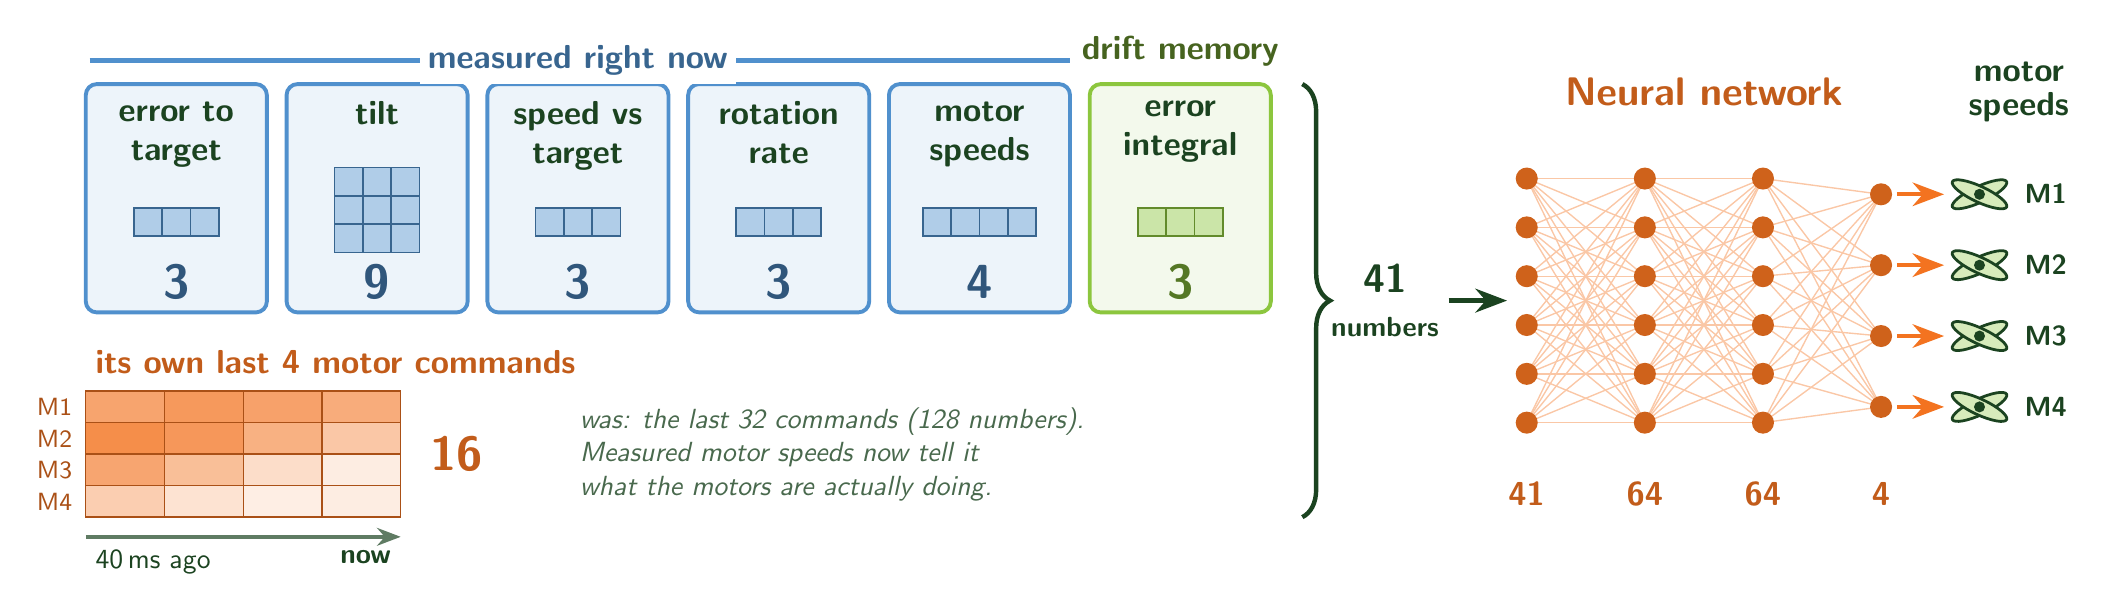
\begin{tikzpicture}
  % ---------- the "right now" groups as cards ----------
  \foreach \x/\ttl/\n/\col in {
      0/{error to\\target}/3/bleu,
      2.55/{tilt}/9/bleu,
      5.1/{speed vs\\target}/3/bleu,
      7.65/{rotation\\rate}/3/bleu,
      10.2/{motor\\speeds}/4/bleu,
      12.75/{error\\integral}/3/vert} {
    \draw[card=\col] (\x-1.15,-1.45) rectangle (\x+1.15,1.45);
    \node[align=center, font=\large\bfseries, text=saclaydk, anchor=north] at (\x,1.35) {\ttl};
    \node[font=\LARGE\bfseries, text=\col!60!black, anchor=south] at (\x,-1.4) {\n};
  }
  % cells inside the cards
  \foreach \x in {0,5.1,7.65} \foreach \i in {-1,0,1}
    \draw[cell=bleu] (\x+\i*\s-\s/2,-0.3-\s/2) rectangle ++(\s,\s);
  \foreach \i in {-1,0,1} \foreach \j in {-1,0,1}
    \draw[cell=bleu] (2.55+\i*\s-\s/2,-0.15+\j*\s-\s/2) rectangle ++(\s,\s);
  \foreach \i in {-1.5,-0.5,0.5,1.5}
    \draw[cell=bleu] (10.2+\i*\s-\s/2,-0.3-\s/2) rectangle ++(\s,\s);
  \foreach \i in {-1,0,1}
    \draw[cell=vert] (12.75+\i*\s-\s/2,-0.3-\s/2) rectangle ++(\s,\s);

  % group headers
  \draw[bleu, line width=1.6pt] (-1.1,1.75) -- (11.35,1.75);
  \node[font=\large\bfseries, text=bleu!70!black, fill=white, inner sep=3pt] at (5.1,1.75) {measured right now};
  \node[font=\large\bfseries, text=vert!50!black, anchor=south] at (12.75,1.55) {drift memory};

  \ifnum\histlen>0
    % ---------- memory: its own last few commands ----------
    \pgfmathtruncatemacro{\nh}{\histlen}
    \pgfmathtruncatemacro{\nnum}{4*\histlen}
    \pgfmathtruncatemacro{\ms}{10*\histlen}
    \def\gw{1.0}
    \node[anchor=south west, font=\large\bfseries, text=mandarine!80!black] at (-1.15,-2.35)
         {its own last \nh\ motor commands};
    \foreach \c in {1,...,\nh} \foreach \r in {0,...,3} {
      \pgfmathtruncatemacro{\v}{max(12, min(85, 45 + 25*sin(\c*23 + \r*70) + 12*sin(\c*61 + \r*20)))}
      \draw[draw=mandarine!70!black, line width=0.5pt, fill=mandarine!\v]
        (-1.15+\c*\gw-\gw, -2.45-\r*0.4) rectangle ++(\gw, -0.4);
    }
    \node[anchor=west, font=\LARGE\bfseries, text=mandarine!80!black] at (-1.15+\nh*\gw+0.25,-3.25) {\nnum};
    \foreach \r/\m in {0/1,1/2,2/3,3/4}
      \node[font=\small, text=mandarine!70!black, anchor=east] at (-1.2,-2.65-\r*0.4) {M\m};
    \draw[-{Stealth[length=3mm]}, line width=1.4pt, saclaydk!70] (-1.15,-4.3) -- (-1.15+\nh*\gw,-4.3);
    \node[anchor=north west, font=\normalsize, text=saclaydk] at (-1.15,-4.35) {\ms\,ms ago};
    \node[anchor=north east, font=\normalsize\bfseries, text=saclaydk] at (-1.15+\nh*\gw,-4.35) {now};
    \node[anchor=west, align=left, font=\normalsize\itshape, text=saclaydk!80] at (5.0,-3.25)
         {was: the last 32 commands (128 numbers).\\Measured motor speeds now tell it\\what the motors are actually doing.};
    \def\ybot{-4.05}
    \def\ny{-1.3}
  \else
    \node[anchor=north west, align=left, font=\normalsize\itshape, text=saclaydk!80] at (-1.15,-1.8)
         {No memory of its own commands (was: the last 32 = 128 numbers).\\
          Measured motor speeds tell it what the motors are actually doing.};
    \def\ybot{-1.45}
    \def\ny{0}
  \fi
  \pgfmathtruncatemacro{\total}{22 + 4*\histlen + 3}

  % ---------- bracket into the network ----------
  \draw[decorate, decoration={brace, amplitude=10pt}, line width=1.6pt, saclaydk]
    (14.3,1.45) -- (14.3,\ybot);
  \node[font=\Large\bfseries, text=saclaydk, align=center] (tot) at (15.35,\ny) {\total\\[-2pt]{\normalsize numbers}};
  \draw[arr, saclaydk] (tot.east) -- (16.9,\ny);

  % ---------- network ----------
  \pgfmathtruncatemacro{\nin}{\histlen > 0 ? 6 : 5}
  \foreach \L/\x/\n/\sp in {0/17.15/\nin/0.62, 1/18.65/6/0.62, 2/20.15/6/0.62, 3/21.65/4/0.9} {
    \foreach \k in {1,...,\n} \coordinate (N\L-\k) at (\x, {\ny + (\n+1)/2*\sp - \k*\sp});
  }
  \foreach \a/\na/\b/\nb in {0/\nin/1/6, 1/6/2/6, 2/6/3/4}
    \foreach \i in {1,...,\na} \foreach \j in {1,...,\nb}
      \draw[mandarine!40, line width=0.5pt] (N\a-\i) -- (N\b-\j);
  \foreach \L/\n in {0/\nin,1/6,2/6,3/4} \foreach \k in {1,...,\n}
    \fill[mandarine!85!black] (N\L-\k) circle (0.14);
  \foreach \x/\lab in {17.15/\total, 18.65/64, 20.15/64, 21.65/4}
    \node[font=\large\bfseries, text=mandarine!80!black] at (\x,\ny-2.45) {\lab};
  \node[font=\Large\bfseries, text=mandarine!80!black] at (19.4,\ny+2.65) {Neural network};

  % ---------- outputs: 4 propellers ----------
  \foreach \k in {1,...,4} {
    \coordinate (P) at ($(N3-\k)+(1.25,0)$);
    \draw[arr, mandarine, line width=1.4pt] ($(N3-\k)+(0.2,0)$) -- ($(P)+(-0.45,0)$);
    \draw[saclaydk, fill=vert!35, line width=1pt, rotate around={25:(P)}] (P) ellipse (0.38 and 0.1);
    \draw[saclaydk, fill=vert!35, line width=1pt, rotate around={-25:(P)}] (P) ellipse (0.38 and 0.1);
    \fill[saclaydk] (P) circle (0.07);
    \node[anchor=west, font=\normalsize\bfseries, text=saclaydk] at ($(P)+(0.45,0)$) {M\k};
  }
  \node[align=center, font=\large\bfseries, text=saclaydk] at (23.4,\ny+2.65) {motor\\[-2pt]speeds};
\end{tikzpicture}
\end{document}
"   (25 inputs)
% Compiled on its own it gives the 4-step version. In the poster:
%   \includegraphics[width=\linewidth]{images/fig_inputs_short_poster.pdf}
\documentclass[12pt, border=4pt]{standalone}
\usepackage{tikz}
\usetikzlibrary{arrows.meta,positioning,calc,decorations.pathreplacing}
\renewcommand{\familydefault}{\sfdefault}

\definecolor{saclaydk}{RGB}{27,67,32}
\definecolor{mandarine}{RGB}{243,115,32}
\definecolor{vert}{RGB}{140,198,62}
\definecolor{bleu}{RGB}{80,144,205}
\definecolor{rouge}{RGB}{198,11,70}

\tikzset{
  cell/.style={draw=#1!70!black, fill=#1!45, line width=0.6pt},
  card/.style={draw=#1, fill=#1!10, rounded corners=4pt, line width=1.4pt},
  arr/.style={-{Stealth[length=4mm,width=3mm]}, line width=2pt},
}
\newcommand{\s}{0.36} % cell size
\providecommand{\histlen}{4}

\begin{document}
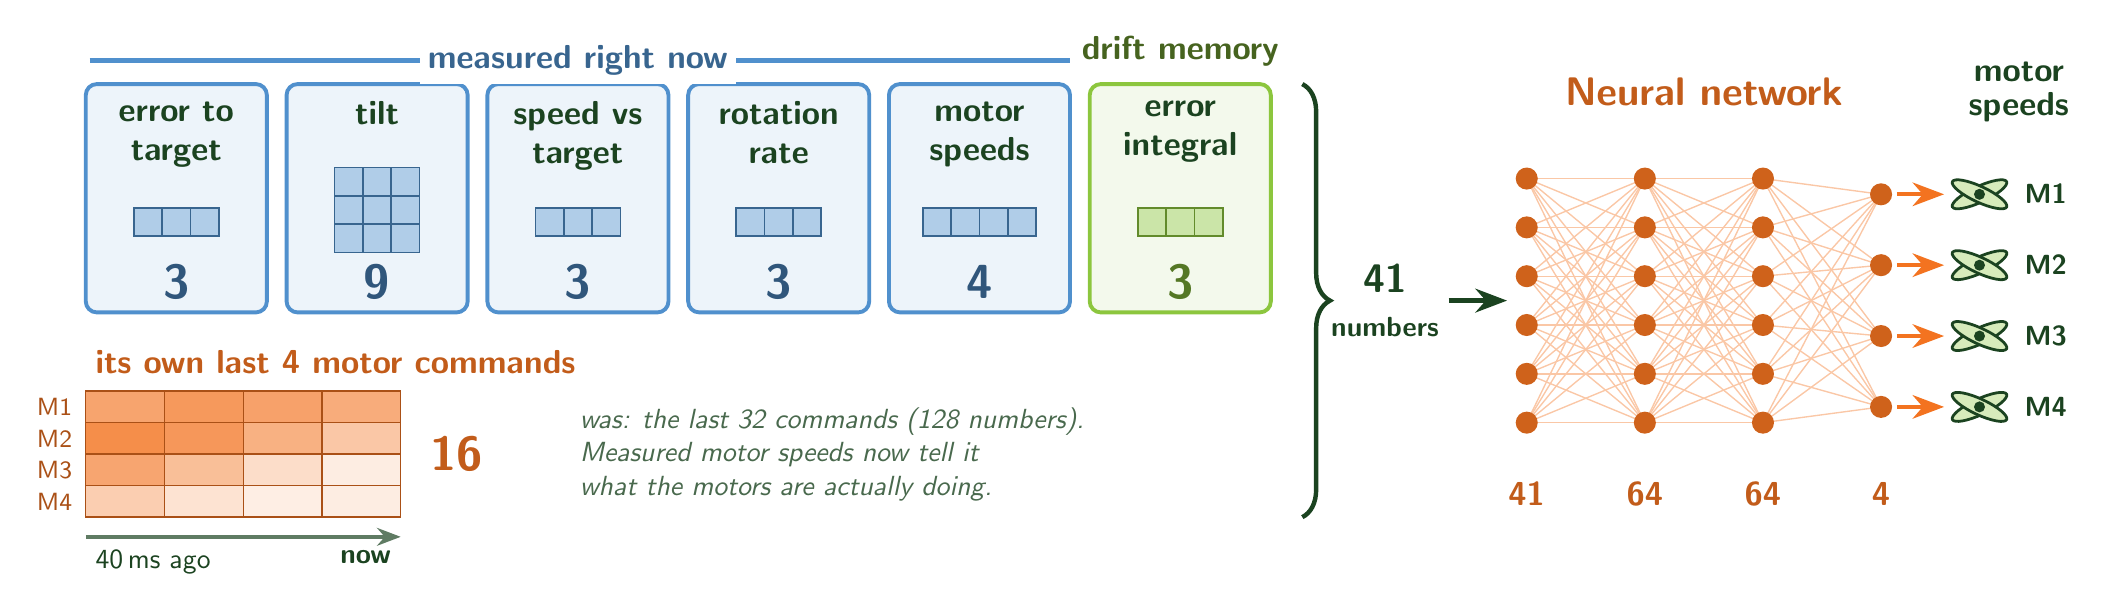
\begin{tikzpicture}
  % ---------- the "right now" groups as cards ----------
  \foreach \x/\ttl/\n/\col in {
      0/{error to\\target}/3/bleu,
      2.55/{tilt}/9/bleu,
      5.1/{speed vs\\target}/3/bleu,
      7.65/{rotation\\rate}/3/bleu,
      10.2/{motor\\speeds}/4/bleu,
      12.75/{error\\integral}/3/vert} {
    \draw[card=\col] (\x-1.15,-1.45) rectangle (\x+1.15,1.45);
    \node[align=center, font=\large\bfseries, text=saclaydk, anchor=north] at (\x,1.35) {\ttl};
    \node[font=\LARGE\bfseries, text=\col!60!black, anchor=south] at (\x,-1.4) {\n};
  }
  % cells inside the cards
  \foreach \x in {0,5.1,7.65} \foreach \i in {-1,0,1}
    \draw[cell=bleu] (\x+\i*\s-\s/2,-0.3-\s/2) rectangle ++(\s,\s);
  \foreach \i in {-1,0,1} \foreach \j in {-1,0,1}
    \draw[cell=bleu] (2.55+\i*\s-\s/2,-0.15+\j*\s-\s/2) rectangle ++(\s,\s);
  \foreach \i in {-1.5,-0.5,0.5,1.5}
    \draw[cell=bleu] (10.2+\i*\s-\s/2,-0.3-\s/2) rectangle ++(\s,\s);
  \foreach \i in {-1,0,1}
    \draw[cell=vert] (12.75+\i*\s-\s/2,-0.3-\s/2) rectangle ++(\s,\s);

  % group headers
  \draw[bleu, line width=1.6pt] (-1.1,1.75) -- (11.35,1.75);
  \node[font=\large\bfseries, text=bleu!70!black, fill=white, inner sep=3pt] at (5.1,1.75) {measured right now};
  \node[font=\large\bfseries, text=vert!50!black, anchor=south] at (12.75,1.55) {drift memory};

  \ifnum\histlen>0
    % ---------- memory: its own last few commands ----------
    \pgfmathtruncatemacro{\nh}{\histlen}
    \pgfmathtruncatemacro{\nnum}{4*\histlen}
    \pgfmathtruncatemacro{\ms}{10*\histlen}
    \def\gw{1.0}
    \node[anchor=south west, font=\large\bfseries, text=mandarine!80!black] at (-1.15,-2.35)
         {its own last \nh\ motor commands};
    \foreach \c in {1,...,\nh} \foreach \r in {0,...,3} {
      \pgfmathtruncatemacro{\v}{max(12, min(85, 45 + 25*sin(\c*23 + \r*70) + 12*sin(\c*61 + \r*20)))}
      \draw[draw=mandarine!70!black, line width=0.5pt, fill=mandarine!\v]
        (-1.15+\c*\gw-\gw, -2.45-\r*0.4) rectangle ++(\gw, -0.4);
    }
    \node[anchor=west, font=\LARGE\bfseries, text=mandarine!80!black] at (-1.15+\nh*\gw+0.25,-3.25) {\nnum};
    \foreach \r/\m in {0/1,1/2,2/3,3/4}
      \node[font=\small, text=mandarine!70!black, anchor=east] at (-1.2,-2.65-\r*0.4) {M\m};
    \draw[-{Stealth[length=3mm]}, line width=1.4pt, saclaydk!70] (-1.15,-4.3) -- (-1.15+\nh*\gw,-4.3);
    \node[anchor=north west, font=\normalsize, text=saclaydk] at (-1.15,-4.35) {\ms\,ms ago};
    \node[anchor=north east, font=\normalsize\bfseries, text=saclaydk] at (-1.15+\nh*\gw,-4.35) {now};
    \node[anchor=west, align=left, font=\normalsize\itshape, text=saclaydk!80] at (5.0,-3.25)
         {was: the last 32 commands (128 numbers).\\Measured motor speeds now tell it\\what the motors are actually doing.};
    \def\ybot{-4.05}
    \def\ny{-1.3}
  \else
    \node[anchor=north west, align=left, font=\normalsize\itshape, text=saclaydk!80] at (-1.15,-1.8)
         {No memory of its own commands (was: the last 32 = 128 numbers).\\
          Measured motor speeds tell it what the motors are actually doing.};
    \def\ybot{-1.45}
    \def\ny{0}
  \fi
  \pgfmathtruncatemacro{\total}{22 + 4*\histlen + 3}

  % ---------- bracket into the network ----------
  \draw[decorate, decoration={brace, amplitude=10pt}, line width=1.6pt, saclaydk]
    (14.3,1.45) -- (14.3,\ybot);
  \node[font=\Large\bfseries, text=saclaydk, align=center] (tot) at (15.35,\ny) {\total\\[-2pt]{\normalsize numbers}};
  \draw[arr, saclaydk] (tot.east) -- (16.9,\ny);

  % ---------- network ----------
  \pgfmathtruncatemacro{\nin}{\histlen > 0 ? 6 : 5}
  \foreach \L/\x/\n/\sp in {0/17.15/\nin/0.62, 1/18.65/6/0.62, 2/20.15/6/0.62, 3/21.65/4/0.9} {
    \foreach \k in {1,...,\n} \coordinate (N\L-\k) at (\x, {\ny + (\n+1)/2*\sp - \k*\sp});
  }
  \foreach \a/\na/\b/\nb in {0/\nin/1/6, 1/6/2/6, 2/6/3/4}
    \foreach \i in {1,...,\na} \foreach \j in {1,...,\nb}
      \draw[mandarine!40, line width=0.5pt] (N\a-\i) -- (N\b-\j);
  \foreach \L/\n in {0/\nin,1/6,2/6,3/4} \foreach \k in {1,...,\n}
    \fill[mandarine!85!black] (N\L-\k) circle (0.14);
  \foreach \x/\lab in {17.15/\total, 18.65/64, 20.15/64, 21.65/4}
    \node[font=\large\bfseries, text=mandarine!80!black] at (\x,\ny-2.45) {\lab};
  \node[font=\Large\bfseries, text=mandarine!80!black] at (19.4,\ny+2.65) {Neural network};

  % ---------- outputs: 4 propellers ----------
  \foreach \k in {1,...,4} {
    \coordinate (P) at ($(N3-\k)+(1.25,0)$);
    \draw[arr, mandarine, line width=1.4pt] ($(N3-\k)+(0.2,0)$) -- ($(P)+(-0.45,0)$);
    \draw[saclaydk, fill=vert!35, line width=1pt, rotate around={25:(P)}] (P) ellipse (0.38 and 0.1);
    \draw[saclaydk, fill=vert!35, line width=1pt, rotate around={-25:(P)}] (P) ellipse (0.38 and 0.1);
    \fill[saclaydk] (P) circle (0.07);
    \node[anchor=west, font=\normalsize\bfseries, text=saclaydk] at ($(P)+(0.45,0)$) {M\k};
  }
  \node[align=center, font=\large\bfseries, text=saclaydk] at (23.4,\ny+2.65) {motor\\[-2pt]speeds};
\end{tikzpicture}
\end{document}
"   (25 inputs)
% Compiled on its own it gives the 4-step version. In the poster:
%   \includegraphics[width=\linewidth]{images/fig_inputs_short_poster.pdf}
\documentclass[12pt, border=4pt]{standalone}
\usepackage{tikz}
\usetikzlibrary{arrows.meta,positioning,calc,decorations.pathreplacing}
\renewcommand{\familydefault}{\sfdefault}

\definecolor{saclaydk}{RGB}{27,67,32}
\definecolor{mandarine}{RGB}{243,115,32}
\definecolor{vert}{RGB}{140,198,62}
\definecolor{bleu}{RGB}{80,144,205}
\definecolor{rouge}{RGB}{198,11,70}

\tikzset{
  cell/.style={draw=#1!70!black, fill=#1!45, line width=0.6pt},
  card/.style={draw=#1, fill=#1!10, rounded corners=4pt, line width=1.4pt},
  arr/.style={-{Stealth[length=4mm,width=3mm]}, line width=2pt},
}
\newcommand{\s}{0.36} % cell size
\providecommand{\histlen}{4}

\begin{document}
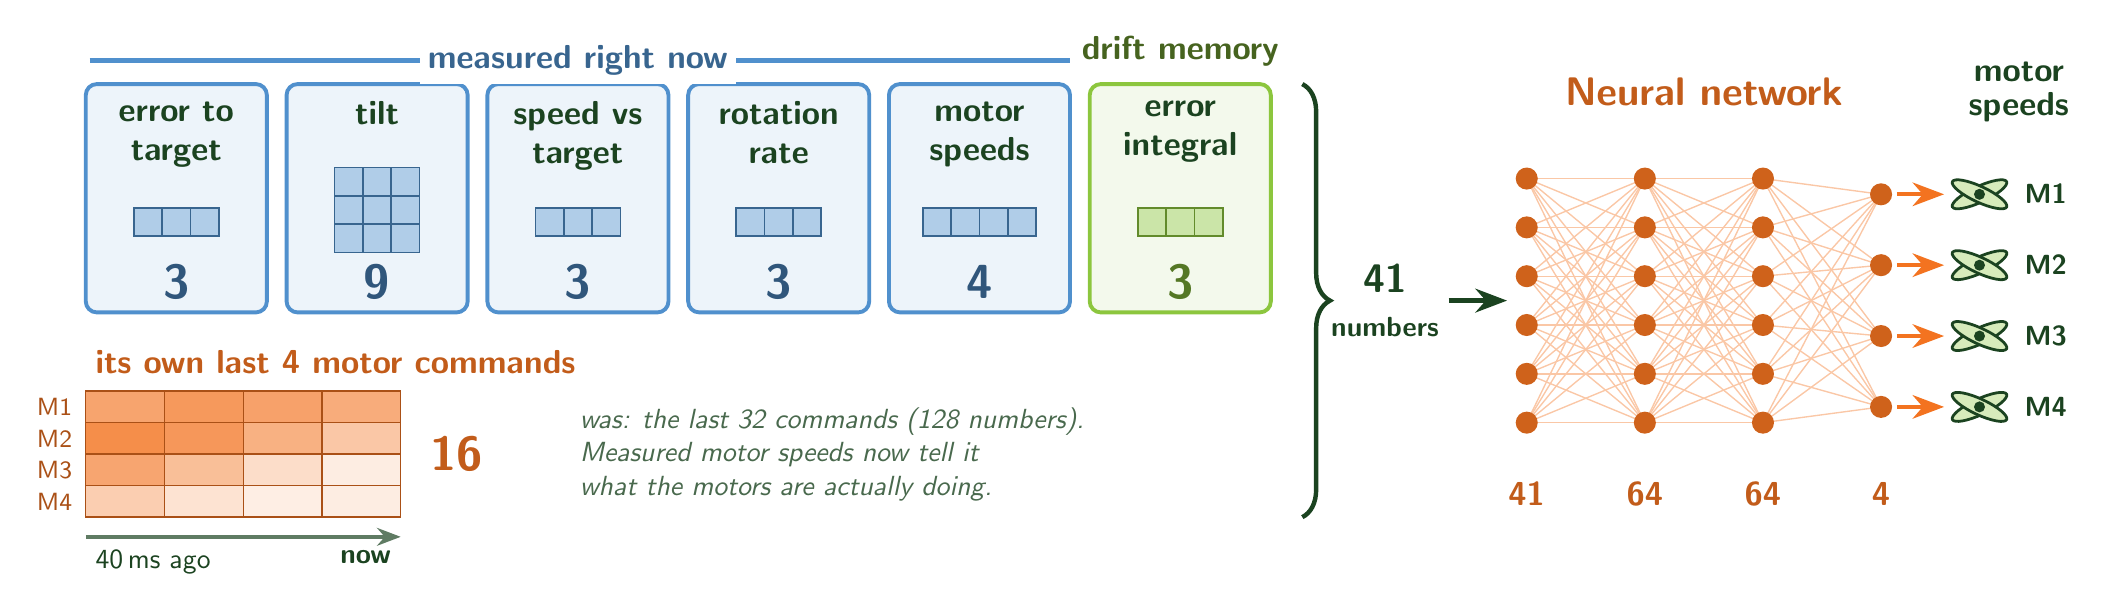
\begin{tikzpicture}
  % ---------- the "right now" groups as cards ----------
  \foreach \x/\ttl/\n/\col in {
      0/{error to\\target}/3/bleu,
      2.55/{tilt}/9/bleu,
      5.1/{speed vs\\target}/3/bleu,
      7.65/{rotation\\rate}/3/bleu,
      10.2/{motor\\speeds}/4/bleu,
      12.75/{error\\integral}/3/vert} {
    \draw[card=\col] (\x-1.15,-1.45) rectangle (\x+1.15,1.45);
    \node[align=center, font=\large\bfseries, text=saclaydk, anchor=north] at (\x,1.35) {\ttl};
    \node[font=\LARGE\bfseries, text=\col!60!black, anchor=south] at (\x,-1.4) {\n};
  }
  % cells inside the cards
  \foreach \x in {0,5.1,7.65} \foreach \i in {-1,0,1}
    \draw[cell=bleu] (\x+\i*\s-\s/2,-0.3-\s/2) rectangle ++(\s,\s);
  \foreach \i in {-1,0,1} \foreach \j in {-1,0,1}
    \draw[cell=bleu] (2.55+\i*\s-\s/2,-0.15+\j*\s-\s/2) rectangle ++(\s,\s);
  \foreach \i in {-1.5,-0.5,0.5,1.5}
    \draw[cell=bleu] (10.2+\i*\s-\s/2,-0.3-\s/2) rectangle ++(\s,\s);
  \foreach \i in {-1,0,1}
    \draw[cell=vert] (12.75+\i*\s-\s/2,-0.3-\s/2) rectangle ++(\s,\s);

  % group headers
  \draw[bleu, line width=1.6pt] (-1.1,1.75) -- (11.35,1.75);
  \node[font=\large\bfseries, text=bleu!70!black, fill=white, inner sep=3pt] at (5.1,1.75) {measured right now};
  \node[font=\large\bfseries, text=vert!50!black, anchor=south] at (12.75,1.55) {drift memory};

  \ifnum\histlen>0
    % ---------- memory: its own last few commands ----------
    \pgfmathtruncatemacro{\nh}{\histlen}
    \pgfmathtruncatemacro{\nnum}{4*\histlen}
    \pgfmathtruncatemacro{\ms}{10*\histlen}
    \def\gw{1.0}
    \node[anchor=south west, font=\large\bfseries, text=mandarine!80!black] at (-1.15,-2.35)
         {its own last \nh\ motor commands};
    \foreach \c in {1,...,\nh} \foreach \r in {0,...,3} {
      \pgfmathtruncatemacro{\v}{max(12, min(85, 45 + 25*sin(\c*23 + \r*70) + 12*sin(\c*61 + \r*20)))}
      \draw[draw=mandarine!70!black, line width=0.5pt, fill=mandarine!\v]
        (-1.15+\c*\gw-\gw, -2.45-\r*0.4) rectangle ++(\gw, -0.4);
    }
    \node[anchor=west, font=\LARGE\bfseries, text=mandarine!80!black] at (-1.15+\nh*\gw+0.25,-3.25) {\nnum};
    \foreach \r/\m in {0/1,1/2,2/3,3/4}
      \node[font=\small, text=mandarine!70!black, anchor=east] at (-1.2,-2.65-\r*0.4) {M\m};
    \draw[-{Stealth[length=3mm]}, line width=1.4pt, saclaydk!70] (-1.15,-4.3) -- (-1.15+\nh*\gw,-4.3);
    \node[anchor=north west, font=\normalsize, text=saclaydk] at (-1.15,-4.35) {\ms\,ms ago};
    \node[anchor=north east, font=\normalsize\bfseries, text=saclaydk] at (-1.15+\nh*\gw,-4.35) {now};
    \node[anchor=west, align=left, font=\normalsize\itshape, text=saclaydk!80] at (5.0,-3.25)
         {was: the last 32 commands (128 numbers).\\Measured motor speeds now tell it\\what the motors are actually doing.};
    \def\ybot{-4.05}
    \def\ny{-1.3}
  \else
    \node[anchor=north west, align=left, font=\normalsize\itshape, text=saclaydk!80] at (-1.15,-1.8)
         {No memory of its own commands (was: the last 32 = 128 numbers).\\
          Measured motor speeds tell it what the motors are actually doing.};
    \def\ybot{-1.45}
    \def\ny{0}
  \fi
  \pgfmathtruncatemacro{\total}{22 + 4*\histlen + 3}

  % ---------- bracket into the network ----------
  \draw[decorate, decoration={brace, amplitude=10pt}, line width=1.6pt, saclaydk]
    (14.3,1.45) -- (14.3,\ybot);
  \node[font=\Large\bfseries, text=saclaydk, align=center] (tot) at (15.35,\ny) {\total\\[-2pt]{\normalsize numbers}};
  \draw[arr, saclaydk] (tot.east) -- (16.9,\ny);

  % ---------- network ----------
  \pgfmathtruncatemacro{\nin}{\histlen > 0 ? 6 : 5}
  \foreach \L/\x/\n/\sp in {0/17.15/\nin/0.62, 1/18.65/6/0.62, 2/20.15/6/0.62, 3/21.65/4/0.9} {
    \foreach \k in {1,...,\n} \coordinate (N\L-\k) at (\x, {\ny + (\n+1)/2*\sp - \k*\sp});
  }
  \foreach \a/\na/\b/\nb in {0/\nin/1/6, 1/6/2/6, 2/6/3/4}
    \foreach \i in {1,...,\na} \foreach \j in {1,...,\nb}
      \draw[mandarine!40, line width=0.5pt] (N\a-\i) -- (N\b-\j);
  \foreach \L/\n in {0/\nin,1/6,2/6,3/4} \foreach \k in {1,...,\n}
    \fill[mandarine!85!black] (N\L-\k) circle (0.14);
  \foreach \x/\lab in {17.15/\total, 18.65/64, 20.15/64, 21.65/4}
    \node[font=\large\bfseries, text=mandarine!80!black] at (\x,\ny-2.45) {\lab};
  \node[font=\Large\bfseries, text=mandarine!80!black] at (19.4,\ny+2.65) {Neural network};

  % ---------- outputs: 4 propellers ----------
  \foreach \k in {1,...,4} {
    \coordinate (P) at ($(N3-\k)+(1.25,0)$);
    \draw[arr, mandarine, line width=1.4pt] ($(N3-\k)+(0.2,0)$) -- ($(P)+(-0.45,0)$);
    \draw[saclaydk, fill=vert!35, line width=1pt, rotate around={25:(P)}] (P) ellipse (0.38 and 0.1);
    \draw[saclaydk, fill=vert!35, line width=1pt, rotate around={-25:(P)}] (P) ellipse (0.38 and 0.1);
    \fill[saclaydk] (P) circle (0.07);
    \node[anchor=west, font=\normalsize\bfseries, text=saclaydk] at ($(P)+(0.45,0)$) {M\k};
  }
  \node[align=center, font=\large\bfseries, text=saclaydk] at (23.4,\ny+2.65) {motor\\[-2pt]speeds};
\end{tikzpicture}
\end{document}
"   (25 inputs)
% Compiled on its own it gives the 4-step version. In the poster:
%   \includegraphics[width=\linewidth]{images/fig_inputs_short_poster.pdf}
\documentclass[12pt, border=4pt]{standalone}
\usepackage{tikz}
\usetikzlibrary{arrows.meta,positioning,calc,decorations.pathreplacing}
\renewcommand{\familydefault}{\sfdefault}

\definecolor{saclaydk}{RGB}{27,67,32}
\definecolor{mandarine}{RGB}{243,115,32}
\definecolor{vert}{RGB}{140,198,62}
\definecolor{bleu}{RGB}{80,144,205}
\definecolor{rouge}{RGB}{198,11,70}

\tikzset{
  cell/.style={draw=#1!70!black, fill=#1!45, line width=0.6pt},
  card/.style={draw=#1, fill=#1!10, rounded corners=4pt, line width=1.4pt},
  arr/.style={-{Stealth[length=4mm,width=3mm]}, line width=2pt},
}
\newcommand{\s}{0.36} % cell size
\providecommand{\histlen}{4}

\begin{document}
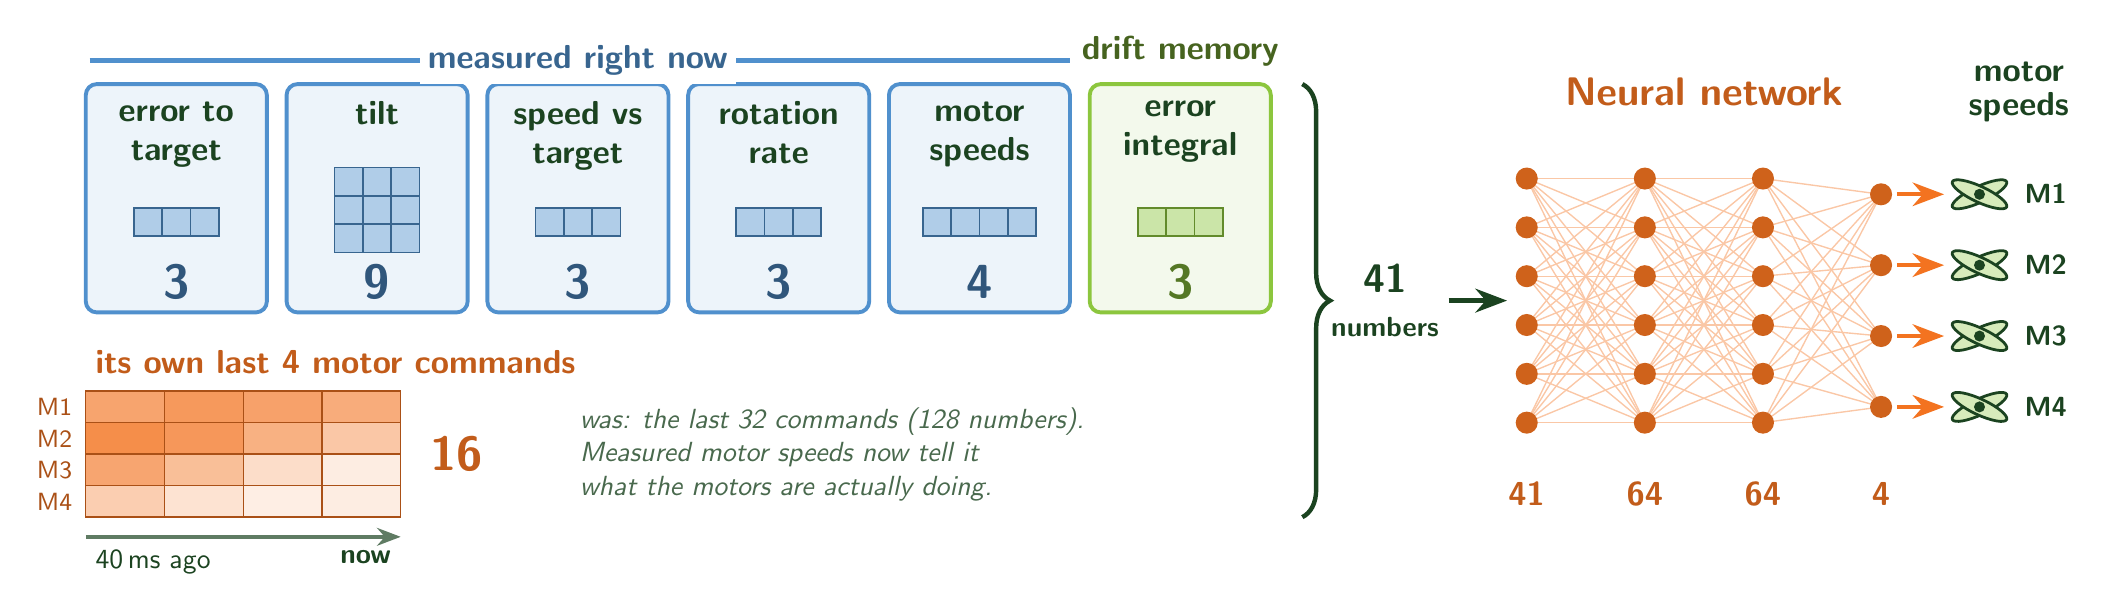
\begin{tikzpicture}
  % ---------- the "right now" groups as cards ----------
  \foreach \x/\ttl/\n/\col in {
      0/{error to\\target}/3/bleu,
      2.55/{tilt}/9/bleu,
      5.1/{speed vs\\target}/3/bleu,
      7.65/{rotation\\rate}/3/bleu,
      10.2/{motor\\speeds}/4/bleu,
      12.75/{error\\integral}/3/vert} {
    \draw[card=\col] (\x-1.15,-1.45) rectangle (\x+1.15,1.45);
    \node[align=center, font=\large\bfseries, text=saclaydk, anchor=north] at (\x,1.35) {\ttl};
    \node[font=\LARGE\bfseries, text=\col!60!black, anchor=south] at (\x,-1.4) {\n};
  }
  % cells inside the cards
  \foreach \x in {0,5.1,7.65} \foreach \i in {-1,0,1}
    \draw[cell=bleu] (\x+\i*\s-\s/2,-0.3-\s/2) rectangle ++(\s,\s);
  \foreach \i in {-1,0,1} \foreach \j in {-1,0,1}
    \draw[cell=bleu] (2.55+\i*\s-\s/2,-0.15+\j*\s-\s/2) rectangle ++(\s,\s);
  \foreach \i in {-1.5,-0.5,0.5,1.5}
    \draw[cell=bleu] (10.2+\i*\s-\s/2,-0.3-\s/2) rectangle ++(\s,\s);
  \foreach \i in {-1,0,1}
    \draw[cell=vert] (12.75+\i*\s-\s/2,-0.3-\s/2) rectangle ++(\s,\s);

  % group headers
  \draw[bleu, line width=1.6pt] (-1.1,1.75) -- (11.35,1.75);
  \node[font=\large\bfseries, text=bleu!70!black, fill=white, inner sep=3pt] at (5.1,1.75) {measured right now};
  \node[font=\large\bfseries, text=vert!50!black, anchor=south] at (12.75,1.55) {drift memory};

  \ifnum\histlen>0
    % ---------- memory: its own last few commands ----------
    \pgfmathtruncatemacro{\nh}{\histlen}
    \pgfmathtruncatemacro{\nnum}{4*\histlen}
    \pgfmathtruncatemacro{\ms}{10*\histlen}
    \def\gw{1.0}
    \node[anchor=south west, font=\large\bfseries, text=mandarine!80!black] at (-1.15,-2.35)
         {its own last \nh\ motor commands};
    \foreach \c in {1,...,\nh} \foreach \r in {0,...,3} {
      \pgfmathtruncatemacro{\v}{max(12, min(85, 45 + 25*sin(\c*23 + \r*70) + 12*sin(\c*61 + \r*20)))}
      \draw[draw=mandarine!70!black, line width=0.5pt, fill=mandarine!\v]
        (-1.15+\c*\gw-\gw, -2.45-\r*0.4) rectangle ++(\gw, -0.4);
    }
    \node[anchor=west, font=\LARGE\bfseries, text=mandarine!80!black] at (-1.15+\nh*\gw+0.25,-3.25) {\nnum};
    \foreach \r/\m in {0/1,1/2,2/3,3/4}
      \node[font=\small, text=mandarine!70!black, anchor=east] at (-1.2,-2.65-\r*0.4) {M\m};
    \draw[-{Stealth[length=3mm]}, line width=1.4pt, saclaydk!70] (-1.15,-4.3) -- (-1.15+\nh*\gw,-4.3);
    \node[anchor=north west, font=\normalsize, text=saclaydk] at (-1.15,-4.35) {\ms\,ms ago};
    \node[anchor=north east, font=\normalsize\bfseries, text=saclaydk] at (-1.15+\nh*\gw,-4.35) {now};
    \node[anchor=west, align=left, font=\normalsize\itshape, text=saclaydk!80] at (5.0,-3.25)
         {was: the last 32 commands (128 numbers).\\Measured motor speeds now tell it\\what the motors are actually doing.};
    \def\ybot{-4.05}
    \def\ny{-1.3}
  \else
    \node[anchor=north west, align=left, font=\normalsize\itshape, text=saclaydk!80] at (-1.15,-1.8)
         {No memory of its own commands (was: the last 32 = 128 numbers).\\
          Measured motor speeds tell it what the motors are actually doing.};
    \def\ybot{-1.45}
    \def\ny{0}
  \fi
  \pgfmathtruncatemacro{\total}{22 + 4*\histlen + 3}

  % ---------- bracket into the network ----------
  \draw[decorate, decoration={brace, amplitude=10pt}, line width=1.6pt, saclaydk]
    (14.3,1.45) -- (14.3,\ybot);
  \node[font=\Large\bfseries, text=saclaydk, align=center] (tot) at (15.35,\ny) {\total\\[-2pt]{\normalsize numbers}};
  \draw[arr, saclaydk] (tot.east) -- (16.9,\ny);

  % ---------- network ----------
  \pgfmathtruncatemacro{\nin}{\histlen > 0 ? 6 : 5}
  \foreach \L/\x/\n/\sp in {0/17.15/\nin/0.62, 1/18.65/6/0.62, 2/20.15/6/0.62, 3/21.65/4/0.9} {
    \foreach \k in {1,...,\n} \coordinate (N\L-\k) at (\x, {\ny + (\n+1)/2*\sp - \k*\sp});
  }
  \foreach \a/\na/\b/\nb in {0/\nin/1/6, 1/6/2/6, 2/6/3/4}
    \foreach \i in {1,...,\na} \foreach \j in {1,...,\nb}
      \draw[mandarine!40, line width=0.5pt] (N\a-\i) -- (N\b-\j);
  \foreach \L/\n in {0/\nin,1/6,2/6,3/4} \foreach \k in {1,...,\n}
    \fill[mandarine!85!black] (N\L-\k) circle (0.14);
  \foreach \x/\lab in {17.15/\total, 18.65/64, 20.15/64, 21.65/4}
    \node[font=\large\bfseries, text=mandarine!80!black] at (\x,\ny-2.45) {\lab};
  \node[font=\Large\bfseries, text=mandarine!80!black] at (19.4,\ny+2.65) {Neural network};

  % ---------- outputs: 4 propellers ----------
  \foreach \k in {1,...,4} {
    \coordinate (P) at ($(N3-\k)+(1.25,0)$);
    \draw[arr, mandarine, line width=1.4pt] ($(N3-\k)+(0.2,0)$) -- ($(P)+(-0.45,0)$);
    \draw[saclaydk, fill=vert!35, line width=1pt, rotate around={25:(P)}] (P) ellipse (0.38 and 0.1);
    \draw[saclaydk, fill=vert!35, line width=1pt, rotate around={-25:(P)}] (P) ellipse (0.38 and 0.1);
    \fill[saclaydk] (P) circle (0.07);
    \node[anchor=west, font=\normalsize\bfseries, text=saclaydk] at ($(P)+(0.45,0)$) {M\k};
  }
  \node[align=center, font=\large\bfseries, text=saclaydk] at (23.4,\ny+2.65) {motor\\[-2pt]speeds};
\end{tikzpicture}
\end{document}
